
\chapter{Non-adiabatic control of quantum energy transfer in ordered and disordered arrays}
\label{ch:wave packet}

An elementary excitation in an aggregate of coupled particles
generates a collective excited state. We show that the dynamics of
these excitations can be controlled by applying a transient external
potential which modifies the phase of the quantum states of the 
individual particles. The method is based on an interplay of
adiabatic and sudden time scales in the quantum evolution of the many-body states. We show that
specific phase transformations can be used to accelerate or
decelerate quantum energy transfer and spatially focus delocalized
excitations onto different parts of  arrays of quantum
particles. {We consider possible experimental implementations of
the proposed technique and study the effect of disorder due to
the presence of impurities on its fidelity. {We further show
that the proposed technique can allow control of energy transfer  in completely disordered systems.}}


\section{Introduction}
\label{sec:energyTransferIntro}

The experiments with ultracold atoms and molecules trapped in optical lattices have opened a new frontier of 
condensed-matter physics research. The unique properties of these systems -- in particular, large ($>$ 400 nm) 
separation of lattice sites, the possibility of tuning the tunnelling amplitude of particles  between lattice sites by
 varying the trapping field and the possibility of controlling interparticle interactions with external electric or 
magnetic fields -- offer many exciting applications ranging from quantum simulation of complex lattice models 
\cite{Kohl2005, Barnett2006, micheli2006, Brennen2007, Buchler2007, McKay2008, Jordens2008, Schneider2008, 
Carr, Carr2, Trefzger2010, Kestner2011, gorshkov, gorshkov2} to the study of novel quasi-particles \cite{biexcitons}
 that cannot be realized in solid-state crystals.
 In the limit of strong trapping field,  each site of an optical lattice is populated by a fixed number of ultracold atoms
 or molecules. 
Such states can be produced with either bosonic or fermionic particles \cite{Greiner2002, Jordens2008}. Here, we consider
 an optical lattice fully or partially filled with one particle per lattice site, and assume that tunnelling between lattice
 sites is completely suppressed. Such an array can be thought of as a prototype  of a  system,
 in which a single lattice site (or a small number of lattice sites) can be individually addressed
by an external field of a focused laser beam. This can be exploited for engineering the properties of quantum 
many-body systems by changing the energy of particles in individual lattice sites \cite{our-2012-prl}.




In the present work, we consider the generic problem of energy transfer -- i.e. the time evolution of an elementary  
quantum excitation -- in such a system. In particular, we explore the possibility of controlling energy transfer through
 an array of coupled quantum monomers by applying monomer-specific external perturbations. This is necessary for 
several applications. First, collective excitations in molecular arrays in optical lattices have been proposed as 
high-fidelity candidates for quantum memory \cite{peter-rabl, peter-rabl2}.  The ability to manipulate collective excitations is necessary
 for building scalable quantum computing networks \cite{quantum-computing}. 
Second, ultracold atoms and 
molecules in optical lattices can be perturbed by a disorder potential with tunable strength 
\cite{anderson-localization-of-ultracold-atoms}. Engineering localized and delocalized excitations in such systems 
can be used to investigate the role of disorder-induced perturbations  on quantum energy transfer, a question of
 central importance for building efficient light-harvesting devices \cite{solar-cell}.
 Third, the possibility of controlling energy transfer in an optical lattice with ultracold atoms or molecules can
 be used to realize inelastic scattering processes with both spatial and temporal control. Finally, control over energy
transfer in quantum systems can be used for studying condensed-matter excitations and energy transport without 
statistical averaging.

An excitation of a coupled many-body system generates a wave packet representing a coherent superposition of 
single-particle excitations. The method proposed here is based on shaping such many-body wave packets by a series
 of sudden perturbations, in analogy with the techniques developed for strong-field alignment and orientation of 
molecules in the gas phase \cite{alignment-review}. Alignment is used in molecular imaging experiments and
 molecular optics \cite{alignment-review, imaging1, imaging2, imaging3}, and is predicted to provide control over 
mechanical properties of molecular scattering \cite{averbukh-AlignedInteractions, averbukh-AlignedInteractions2}. 
Here, we consider the use of similar techniques for controlling quantum energy transfer in an  interacting
 many-body system.
 When applied to a completely ordered system, the proposed method is reminiscent of the techniques used to 
move atoms in optical lattices, where a uniform force is applied for a short period of time \cite{denschlag2002}. 
The conceptual difference comes from the fact that in the present case the momentum is acquired by a 
quasi-particle -- a collective excitation distributed over many monomers. During the subsequent evolution, 
the particles do not move -- rather, the excitation is transferred from one monomer to another. In order to control
 such excitations, we exploit an interplay of the adiabatic and sudden time scales, which correspond to
 single-monomer and multi-monomer evolution. We also exploit the wave-like nature of the excitation wave function
 to draw on the analogy with wave optics. This analogy, too, is not complete due to the discrete nature of the lattice.

In order to emphasize the generality of the proposed method, we formulate the 
problem in terms of the general Hamiltonian parameters. We then describe in detail how the required external 
perturbations can be realized in experiments with ultracold atoms and molecules. The possibility of using rotational 
excitations in molecular arrays is particularly interesting due to the long lifetime of rotationally excited states. 
Electronic excitations of atoms in an optical lattice may also give rise to collective excitations \cite{Zoubi1}. However, the 
lifetime of these excited states is limited by fast spontaneous emission \cite{electronic-exciton1, electronic-exciton2}. We propose a mechanism for 
suppressing spontaneous decay by tailoring the properties of the excitation wave packets. 


The paper has the following structure. \Autoref{sec:phaseKicking} and \autoref{sec:focusing} present the results in terms of the general 
Hamiltonian parameters.  \Autoref{sec:excitationAtomMolecule} addresses the particular case of ultracold atoms and molecules.
\Autoref{sec:controlEnergyTransfer} discusses controlled energy transfer in systems with, specifically, 
dipole - dipole interactions. \Autoref{sec:energyTransferVacancy} considers the effects of lattice vacancies on the possibility of controlling 
energy transfer and \autoref{sec:focusingStrongDisorder} extends the proposed technique to
control of excitation dynamics in strongly disordered arrays with a large
concentration of impurities. \Autoref{sec:energyTransferConclusion} presents the conclusions.

\section{Sudden phase transformation}
\label{sec:phaseKicking}

Consider, first, an ensemble of ${N}$ coupled identical monomers
possessing two internal states arranged in a one-dimensional array
with translational symmetry. The Hamiltonian for such a system is
given by
\begin{equation}
H_{\rm{exc}} = \Delta E_{e-g}\sum_n | e_n \rangle \langle e_n | +
\sum_{n,m} \alpha(n-m) |e_n, g_m\rangle \langle g_n, e_m | \ ,
\label{ham}
\end{equation}
where  $|g_n \rangle$ and $|e_n\rangle$ denote the ground and
excited states in site $n$, $\Delta E_{e-g}$ is the monomer
excitation energy and $\alpha(n-m)$ represents the coupling
between two monomers at sites $n$ and $m$. 
Any singly excited state of the system is given by
%
\begin{eqnarray}
|\psi_{\rm exc}\rangle = \sum_{n=1}^N C_n |e_n\rangle \prod_{i
\neq n} |g_i\rangle . \label{basis}
\end{eqnarray}
%
In general, the expansion coefficients $C_n$ are complicated functions of $n$ determined by the properties of the system, in particular, the translational invariance or lack thereof as well as the strength of disorder potential. 
 If an ideal, periodic system with lattice constant $a$ is excited by a single-photon transition, 
the expansion coefficients are  $C_n =
e^{iakn}/\sqrt{N}$ and  $|\psi_{\rm exc} \rangle \Rightarrow
|k\rangle$ represents a quasi-particle called
Frenkel exciton, characterized by the wave vector $k$
\cite{agranovich}. The magnitude of the wave vector $k$ is determined by the conservation of the total (exciton plus photon) momentum. 
The energy of the exciton is given by $E(k) =
\Delta E_{e-g} + \alpha(k)$ with $\alpha(k) =\sum_n \alpha(n)
e^{-i  a k n}$. In the nearest neighbor approximation,
\begin{eqnarray}
E(k) = \Delta E_{e-g} + 2 \alpha \cos ak, \label{dispersion}
\label{Eexc}
\end{eqnarray}
where $\alpha=\alpha(1)$. 
 
 
 


 
%
%If an ideal, periodic system is excited by a single-photon transition, the resulting state is an exciton with wave vector $k$ determined by the conservation of the total (exciton plus photon) momentum. In the presence of a disorder potential, whether coming from jitter in external fields or from incomplete population of lattice sites, the resulting state is a localized excitation. For atoms and molecules on an optical lattice, a localized excitation can also be placed on a single site (or a small number of sites) by applying a gradient of an external electric or magnetic field and inducing transitions in selected atoms by a pulse of resonant electromagnetic field \cite{demille}. Any localized excitation $| \psi \rangle$ is a coherent superposition of the exciton states $| \psi_{\rm exc}(k)\rangle$ with different $k$:
% In many physical systems, the coupling constant $\alpha(n)$ and the transition energies $\Delta E_{e-g}$ can be perturbed by an external potential.

With atoms or molecules on an optical lattice, it is also possible to generate a localized excitation placed on a single site
 (or a small number of sites) by applying a gradient of an external electric or magnetic field and inducing transitions in
 selected atoms by a pulse of resonant electromagnetic field \cite{demille}. The presence of a disorder potential, 
whether coming from jitter in external fields or from incomplete population of lattice sites,  also results in spatial 
localization. Similar to how \autoref{basis} defines the collective excited states in the basis of lattice sites, 
the same excitation state $|\psi_{\rm exc}\rangle$ can be generally written as a coherent superposition of the exciton states
 $|k\rangle$ with different $k$:

\begin{eqnarray}
| \psi \rangle = \sum_{k} G_k | k \rangle ,
\label{k-rep}
\end{eqnarray}
where $G_k$'s are the fourier transforms of $C_n$'s in \autoref{basis}. 

Control over energy transfer in an ordered array can be achieved
by (i) shifting the exciton wave packets in the momentum
representation (which modifies the group velocity and the shape
evolution of the wave packets) and (ii) focusing the wave packets
in the coordinate representation to produce localized excitations
in an arbitrary part of the lattice. To achieve this, we propose
to apply a series of site-dependent perturbations  that modify the phases of the quantum states of spatially separated monomers. 
These phase transformations change the dynamics of the time evolution of the collective excitations. 
Here we consider the transformations leading to acceleration or deceleration of collective excitations, while   
 the focusing phase transformations are described in \autoref{sec:focusing}. 

\subsection{Group velocity of wave packet}
\label{sec:groupVelocity} 

Before we discuss how to accelerate or decelerate the motion of collective excitations, we first need to figure out 
what determine their propagation behaviors.  It turn out that the propagation behavior of an exciton wave packet can be implied from the exciton dispesion curve. More specifically, the first derivative of the dispersion curve
gives approximately the propagation speed of a wave packet in real space. This can be easily shown by  simple derivations. 

In a perfect crystal, the eigenstates of the system is characterized by a wavevector $k$ and its time evolution is 
determined by $E(k)$ through
\multiline{
\ket{k(t)} &=& e^{-i \frac{E(k)}{\hbar}t}\ket{k(t=0)} \nonumber \\
&=&\frac{1}{\sqrt{N}} \sum_{n} e^{i \left[k a n - \frac{E(k)}{\hbar}t \right]} \ket{n(t=0)} \label{eqn:kState}
}
where $N$ is the number of sites in the crystal and $\ket{n(t=0)}$ represents the state of system in which only site
$n$ is in the excited state. It can see from \autoref{eqn:kState} that the probability at each site is always $1/N$ for 
state $\ket{k}$. So the plane wave $\ket{k}$ doesn't move in real space, which is expected. Different from a plane
 wave state, a wave packet composed of different $\ket{k(t)}$ states is not stationary in real space. This is because
 different $\ket{k(t)}$ components correspond to different energy $E(k)$ thus different evolutions, leading to a 
time-dependent interference pattern in real space. To illustrate this point, we consider a Gaussian wave packet in $k$
space 
\multiline{
\ket{\psi(t)} &=&A \sum_{k} e^{-\frac{(k-k_0)^2}{2\sigma^2_{k}}} \ket{k(t)} \nonumber \\
&=& \frac{A}{\sqrt{N}} \sum_{k} e^{-\frac{(k-k_0)^2}{2\sigma^2_{k}}} \sum_{n} e^{i \left[k a n - \frac{E(k)}{\hbar}t \right]} \ket{n(t=0)} \ ,
}
where $A$ is the normalization constant. 
Expanding $E(k)$ around the point $k=k_0$ and ignoring second and higher-order terms of $(k-k_0)$, and replacing the
 summation over $k$ by integration, we obtain an equation that describes the time-evolution of the wave packet in 
real space:
\multiline{
\ket{\psi(t)} = A^{'}\sum_{n} e^{-\frac{(n-v_{\rm g}t)^2}{2(1/\sigma_{k})^2}}\ket{n(t=0)} \ ,
}
where $A^{'}$ is some constant that normalizes the wavefunction and the group velocity
\oneline{
v_{\rm g} = \frac{1}{\hbar}\left.\frac{d E(k)}{d k}\right|_{k=k_0} \label{eqn:groupVelocity}
}
determines how fast the center of the wave packet moves in real space. Therefore, once the exciton dispersion curve is known, the propagation speed of a wave packet that centered around $k_0$ in momentum space can be calculated from the slope of dispersion curve at $k_0$.

\subsection{Phase kicking in quasimomentum space}

As an example, \autoref{fig:movewave packet} presents an exciton dispersion curve. It can seen  that different
 regions of the dispersion curve have different slopes that correspond to different group velocities. 
Direct optical excitation can create an exciton wave packet which centers around $k\approx 0$ in the $k$ space. 
However, such a wave packet hardly travel in real space as a whole since its group velocity is zero. Based on 
\autoref{fig:movewave packet} , if we want accelerate a $k = 0$ wave packet, a sensible way is to move the 
wave packet to the region near $k=\pi/2$ where the slop of the dispersion curve is deep. Similarly, to decelerate a
 wave packet we should move it to a place where the slop is more shallow. Now the problem of
accelerating/decelerating an exciton wave packet becomes the problem of moving the wave packet  as
a whole in $k$ space. 


\addfigure{
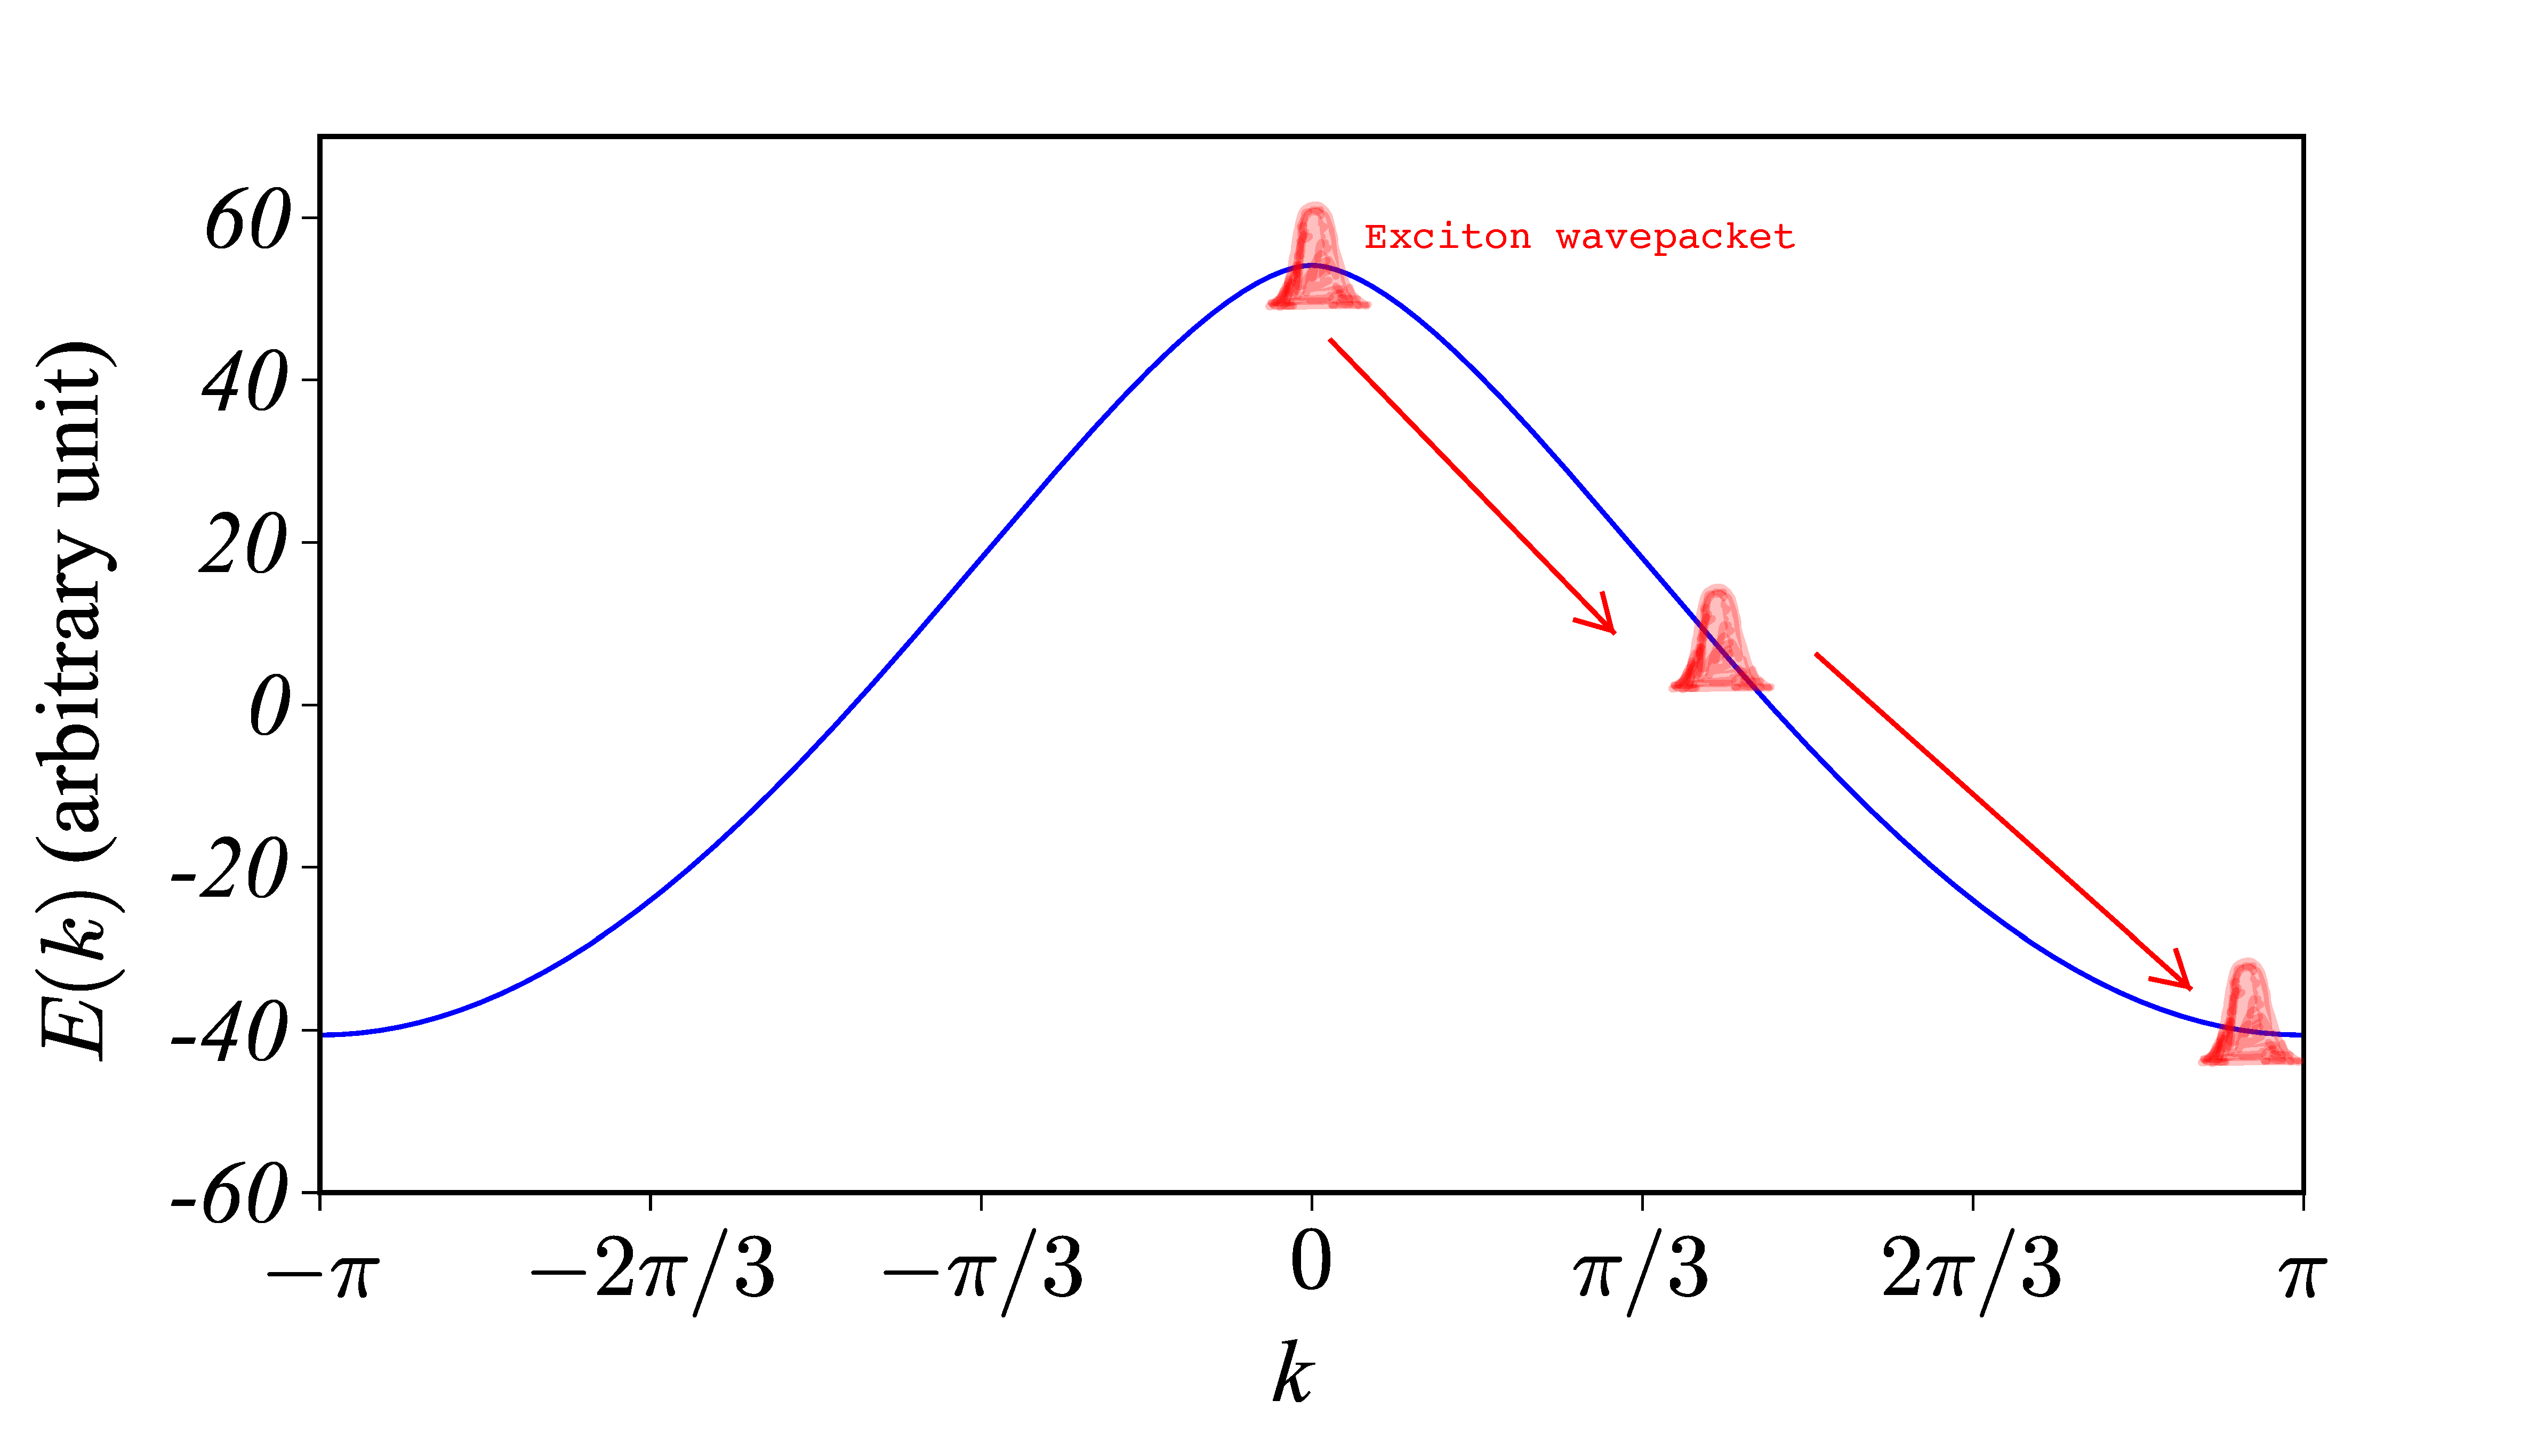
\includegraphics[width=\linewidth]{dispersion-curve-move-wavepacket.png}
\caption{
The dispersion curve of an exciton. The interaction between site $m$ and site $n$ is proportional to $1/|n-m|^3$. 
}
\label{fig:movewave packet}
}


But how do we move an exciton wave packet in $k$ space without changing its shape? We can get some hint from the
expression of the plane wave state
\oneline{
\ket{k(t)} = \frac{1}{\sqrt{N}}\sum_n e^{i k a n} \ket{n(t)} \ . \label{eqn:kStateExpansion}
}
\Autoref{eqn:kStateExpansion} suggests that we can change $\ket{k}$ to $\ket{k+\delta}$ by adding a
 factor $e^{i \delta a n}$ to each term in the expansion.  Since the increment $\delta$ is independent of the $\ket{k}$
state, 
%For modifying the group velocity of a collective excitation, the
%essential idea is to add a factor $e^{i \delta a n}$ to each term
%in the expansion (\ref{basis}), so that 
each $| k\rangle$ component in a wave packet (\autoref{basis}) can be transformed into $|
k+\delta\rangle$ in this way. This transformation shifts the
wave packets by $\delta$ in $k$-space while preserving their
shape. As a result, one can engineer wave packets probing any part
of the dispersion $E(k)$ leading to different group velocity and
shape evolution. 
%The feasibility of such transformation in an ensemble of atoms or molecules on an optical lattice is discussed below and in \autoref{sec:excitationAtomMolecule}. 

Knowing that adding the proper phases is a key step, we now study how to add those phases. There are two
 different time scales involved: one is related to the evolution of the free monomer states, 
$T_m = \hbar/\Delta E_{e-g}$, and the other is related to the excitation population transfer between monomers,
 $T_e = \hbar/\alpha$. Usually, $T_m$ is smaller than $T_e$ by several orders of magnitude. This huge
 difference in magnitude enable us to work with the adiabatic and sudden time scales at the same time as described below. 
%Adding a site-dependent phase to the excitonic wavefunction
%exploits an interplay of the adiabatic and sudden time scales.
Consider  the $n$-th monomer subjected to an external field
$\mathcal{E}_n(t)$ which varies from 0 to some value and then back
to 0 in time $T$. If the variation is adiabatic with respect to
the evolution of the free monomer states, $T\gg T_m$, each eigenstate $|f\rangle$ of the monomer acquires a
state-dependent phase shift \cite{adiabatic-theo}
%
\begin{eqnarray}
\ket{f_n (T)} = e^{-i \phi_{n}^f}\ket{f_n(0)},
\label{adiabatic-theorem} \label{phase}
\end{eqnarray}
%
where $\phi_{n}^f = \frac{1}{\hbar}\int_{0}^{T} E_{n}^f(t )dt$,
$E_{n}^f (t)$ is the instantaneous eigenenergy and $f$ can be $e$
or $g$.
%The operator $\hat{P}_n^\dag = |e_n\rangle\langle g_n |$ acquires the phase $\Phi_n = \phi_{n}^e-\phi_{n}^g$.
Now consider the action of such phase change on the collective
excitation state (\ref{basis}). If $T\ll T_e$, the
change is sudden with respect to the excitation transfer between
monomers, so during the time $T$ the excitation probability doesn't have enough time to propagate 
between different monomers and $C_n$'s in \autoref{basis} remain almost the same. Since $G_k$'s are just fourier
transforms of $C_n$'s, $G_k$ will remain the same as well, conserving the shape of the wave packet $|\psi_{\rm exc}\rangle$ in $k$ space. 
 Then the wave packet $|\psi_{\rm exc}\rangle$ acquires a site-dependent
phase $\Phi_n = \phi_{n}^e-\phi_{n}^g$ that will influence each $\ket{k}$ component in the same way. 
If $\Phi_n = \Phi_0 + n a\delta $, then the momentum $\delta$ is imparted onto the
excitonic wavefunction without changing its shape. By analogy with ``pulsed alignment of
molecules'' \cite{alignment-review}, we call this transformation a
``phase kick'' or ``momentum kick''. Its action is also similar to
that of a thin prism on a wavefront of a monochromatic laser beam.

%%%%%%%%%%%%%%%%%%%%%%%%%%%%%%%%%%%%%%%%%%%%%%%%%%%%%%%%%%%%%%%%%%%%%%%%%%%%%%%%
\begin{figure}[htbp]
\centering
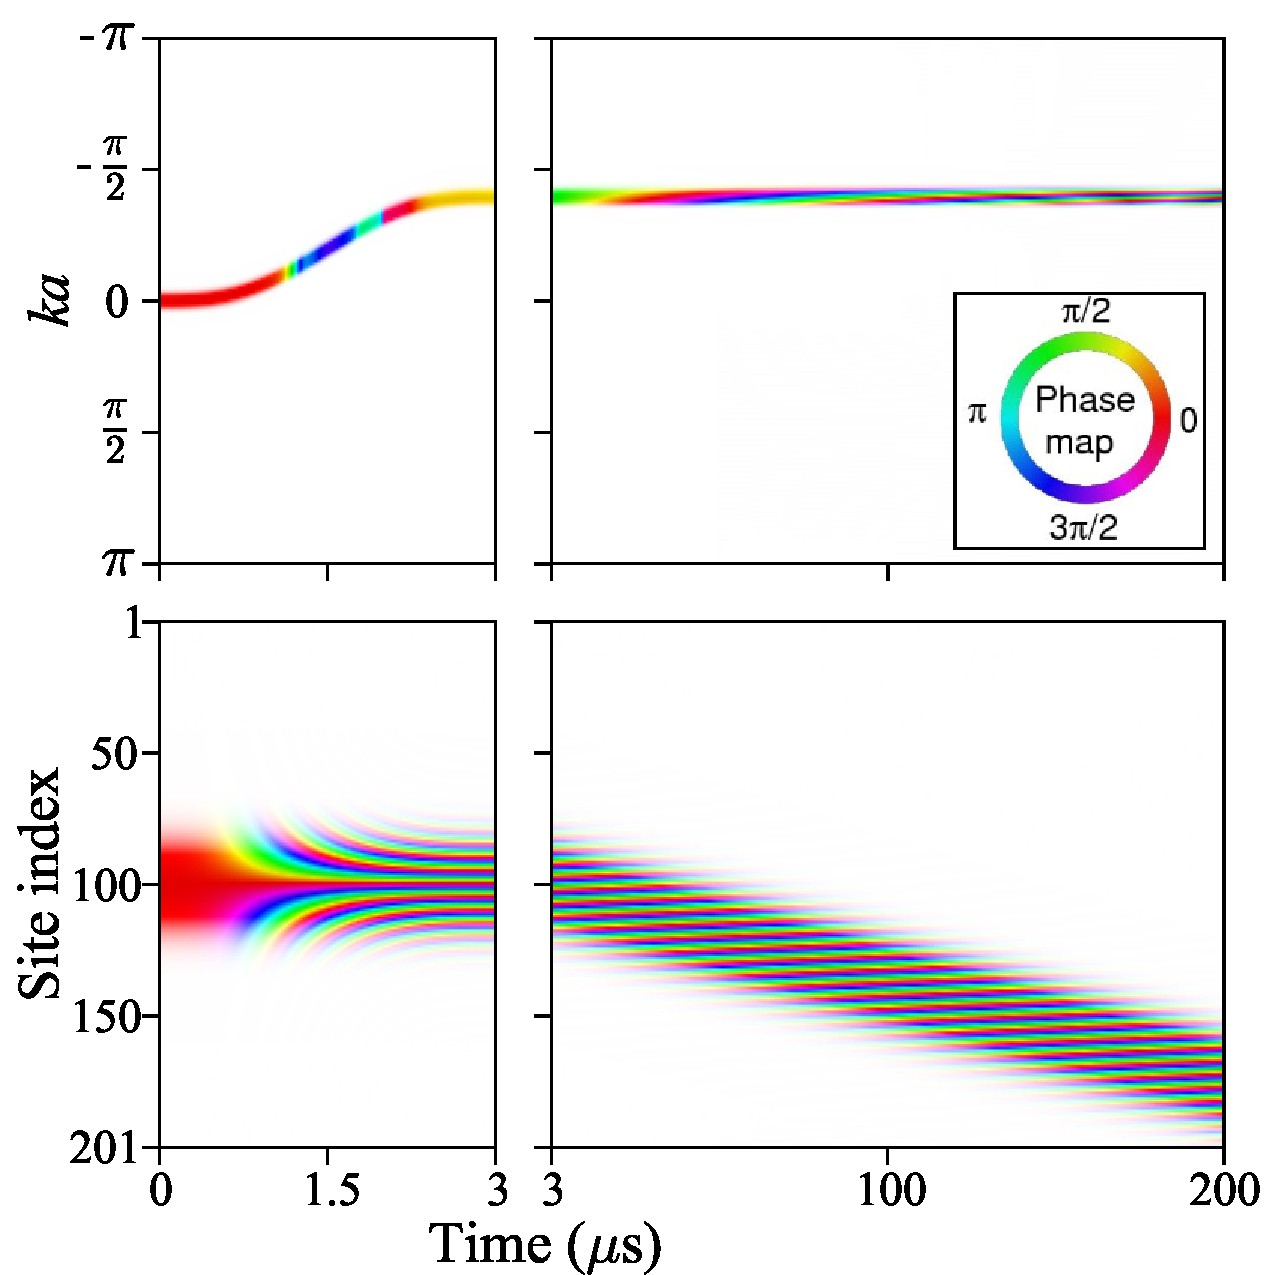
\includegraphics[width=\linewidth]{momentum-kick.pdf}
\caption{
Example of controlled energy transfer in a one-dimensional array of quantum 
monomers subjected to a linear phase transformation. The graph illustrates the evolution of the exciton wave packet  
 centered at $k=0$ and initially positioned at the center of the array. The phase of the wave function
is shown by color.  The brightness of color corresponds to the amplitude of the excitation with white color
 corresponding to zero amplitude. The calculation is for a one-dimensional array
of 201 monomers with $\alpha = 22.83$ kHz and $\Delta E_{e-g} =12.14$ GHz,  and the linear phase transformation 
$\Phi_n \simeq \Phi_0  -1.29 n$. These parameters correspond to LiCs molecules trapped on an optical lattice with lattice constant $a = 400$ nm and
 subjected to a homogeneous DC field of 1 kV/cm directed perpendicular to the
intermolecular axis. The kicking potential leading to this particular  phase transformation  can be provided by a
$\lambda = 1064$ nm Gaussian laser beam, with the propagation direction along the array axis, focused to 5 $\mu$m, 
with the intensity at the focus equal to $10^7$ W/cm$^2$. The laser pulse is on between 0 and  $3 \mu$s.}
\label{momentum-kick}
\end{figure}
%%%%%%%%%%%%%%%%%%%%%%%%%%%%%%%%%%%%%%%%%%%%%%%%%%%%%%%%%%%%%%%%%%%%%%%%%



In order to illustrate the shifting of exciton wave packets in the
momentum space, we solve numerically the time-dependent
Schr\"{o}dinger equation with the unperturbed Hamiltonian
(\ref{ham}),  subjected to a transient site-dependent external
perturbation that temporarily modulates $\Delta E_{e-g}$.
We choose the parameters $\Delta E_{e-g} =12.14\mbox{ GHz}$, $\alpha =22.83\mbox{ kHz}$ and the lattice constant $a=400\mbox{ nm}$ that correspond to an array of
polar molecules trapped in an optical lattice, as described in detail in \autoref{sec:excitationAtomMolecule}.
The time-dependent perturbation has the form of a short pulse with the duration $T = 3\; \mu s$. %$\tb{T} \approx \frac{1}{15} \hbar/\alpha$.
The phase acquired by the particles during this time is given by $\Phi_n \simeq \Phi_0  -1.29 n $, which can be achieved with a focused laser beam, as described in \autoref{sec:excitationAtomMolecule}.



The excitation at $t=0$ is described by
a Gaussian wave packet of the exciton states $|\psi_{\rm
exc}(k)\rangle$, with the central wavevector $k=0$.
\Autoref{momentum-kick} shows that the
entire wave packet acquires momentum during the external perturbation pulse (left
panels). This is manifested as a phase variation in the coordinate
representation, and as a shift of the central momentum in the
$k$-representation. After the external perturbation is gone, the
wave packet does not evolve in the $k$-representation and moves
with the acquired uniform velocity in the coordinate
representation.

The results presented in Figure 1 and all subsequent results of this work are for a single 
collective excitaion in an interacting many-particle system. A general experimental implementation may result in 
multiple excitations, leading to non-linear exciton interactions. There are two mechanisms for exciton - exciton 
interactions: kinematic interactions arising from the statistical properties of excitons and dynamical 
interactions determined by the matrix elements of the inter-particle interactions in the Hilbert sub-space of binary 
excitations \cite{agranovich, marina-bookchapter}. The effects of the kinematic interactions on energy transfer
 in molecular crystals have never been observed so these interactions are considered to be weak, especially in the
 limit of a small number of excitations easily achievable in experiments \cite{kinematic-biexciton-agranovich}. For molecules 
on an optical lattice, the dynamical interactions are important in the presence of strong external electric fields where
 molecular states of different parity are strongly mixed \cite{biexcitons, felipe}.
At weak parity-mixing fields considered here, the exciton-exciton interactions insignificantly mix different $k$ states
 of the individual excitons, contributing weakly  to localization. These effects are expected to be much smaller than
 the disorder-induced perturbations,  discussed in \autoref{sec:energyTransferVacancy}  and \autoref{sec:focusingStrongDisorder}.










\section{Focusing of a delocalized excitation}
\label{sec:focusing}

In order to achieve full control over excitation transfer, it is desirable to find a particular phase transformation
that focuses a delocalized many-body excitation onto a small part of the lattice, ideally a single lattice site.
In optics, a thin lens focuses a collimated light beam by shifting
the phase of the wavefront, thus converting a plane wave to a
converging spherical wave. Similarly, a phase kick can serve as a
time domain ``lens'' for collective excitations: an excitation initially
delocalized over a large number of monomers can be focused onto a
small region of the array after some time. By analogy with optics, a concave or convex
symmetric site-dependent phase $\Phi(n)$ applied simultaneously to
all monomers may turn a broad initial distribution $C_n(t=0)$ into
a narrow one.

The dynamics of the excitation state in the lattice is determined by the time dependence
of the coefficients $C_n(t)$ in  \autoref{basis}. In order to find the expression for $C_n(t)$, we expand the amplitudes
 at $t=0$ in a Fourier series
\begin{eqnarray}
C_n(t=0) = \sum_q
\frac{e^{iq a n}}{\sqrt{N}}C(q; t=0)
\end{eqnarray}
and apply the propagator $e^{-iE(q)t/\hbar}$ to each $q$-component with
$E(q)$ representing the exciton energy given by \autoref{dispersion}.
Transforming the amplitudes $C(q)$ back to the site representation then yields
\begin{equation}
C_m(t) = \frac{1}{N} \sum_{n,k} C_n(t=0) e^{i [\Phi(n) +  k a
(m-n) - E(k) t/\hbar ]},
 \label{Cn(t)}
\end{equation}
where $\Phi(n)$ is a
site-dependent phase applied at $t=0$, as described in the previous section.
Note that the phase $\Phi(n)$ does not have to be applied
instantaneously. The phase  $\Phi(n, t)$ can be applied continuously over an
extended time interval as long as the accumulated phase gives the desired outcome  $\int_0^{T}\Phi(n, t)dt = \Phi(n)$.


\subsection{Focusing to a single site}
\label{sec:singleSiteFocusing}
As \autoref{Cn(t)} shows, the focusing efficiency is determined by the phase transformation and
the shape of the dispersion curve $E(k)$. Given the cosine dispersion of excitons (\ref{dispersion}), is it possible to
 focus a delocalized excitation onto a single lattice site?
To answer this question, we assume an initial condition where the excitation is localized to the site $n_0$, that is,
\multiline{
C_n (t=0) = \delta_{n, n_0} \ ,
}
and run a backward-in-time evolution to calculate the coefficients $C_m(t)$ at $t=-\tau$:
using the expansion of an exponent in Bessel functions (Jacobi-Anger expansion, see Ref. \cite{ jacobi-anger})
\begin{eqnarray}
e^{ia\cos x} = \sum_{n} e^{-i(x-\pi/2)n} J_n(a) \ ,
\end{eqnarray}
we obtain
\multiline{
C_m (-\tau) &=&  \frac{1}{N} \sum_{n,k} C_n(t=0) e^{i [k a
(m-n) - E(k) (-\tau)/\hbar ]} \nonumber \\
&=&  \frac{1}{N} \sum_{n,k} C_n(t=0) e^{i [k a (m-n)}\sum_{n'} e^{- i(ka - \pi/2) n'}  J_{n'}(2\alpha \tau/\hbar) \nonumber \\
&=& \frac{1}{N} \sum_{n,k} \delta_{n, n_0} e^{i [k a (m-n)}\sum_{n'} e^{- i(ka - \pi/2) n'}  J_{n'}(2\alpha \tau/\hbar) \nonumber \\
&=&  \frac{1}{N} \sum_{k} e^{i k a (m-n_0 )}\sum_{n'} e^{- i(ka - \pi/2) n'}  J_{n'}(2\alpha \tau/\hbar) \nonumber \\
&=& \sum_{n'} e^{i\pi n'}  J_{n'}(2\alpha \tau/\hbar) \left( \frac{1}{N}\sum_{k} e^{i k a (m-n_0 - n')}\right) \nonumber \\
&=& \sum_{n'} e^{i\pi n'}  J_{n'}(2\alpha \tau/\hbar) \delta_{n', m-n_0} \nonumber \\
&=& e^{i \pi (m - n_0)/2}J_{m-n_0}\left(2\alpha \tau/\hbar\right) \ , \label{eqn:cosineFocusing}
}
where $J$ is the Bessel function of first kind. 
This  calculation shows that an wavepacket with  the site representation, i.e., 
$C_m(0)= e^{i \pi (m - n_0)/2}J_{m-n_0}\left(2\alpha t/\hbar\right)$,  will focus onto the lattice 
site $n_0$ after evolving for time $t$. We can be easily verify the result by running a forward-in-time evolution
starting with the initial wave packet and making use of 
the orthonormality  of the Bessel functions
\begin{eqnarray}
\sum_{n} J_n(x) J_{n-m}(x) = \delta_{m,0} \ .
\end{eqnarray}
\Autoref{eqn:cosineFocusing} shows that  the focusing of a wave packet onto a
 single site would require not only adding the phase $\Phi(n) = {\rm Arg}[C_m(-\tau)]$, but also the amplitude
 modulations of the coefficients equal to the absolute values of $C_m(-\tau)$. This second task is
 beyond the manipulation tools considered here. However, creating such a wave packet may require multiple and 
complicated phase transformations, which may be difficult to realize in experiments. 


\subsection{Focusing a broad wavepacket in coordinate space}
\label{sec:wavepacketFocusing}

A simpler procedure can be implemented if the phase transformations are restricted to a particular part of
the exciton dispersion.
From wave optics, waves with quadratic dispersion can be
focused, while those with linear dispersion propagate without changing
the wave packet shape \cite{focusing-books-1,focusing-books-2}. It is this interplay of the quadratic (at low $k$) and
 linear (at $k \approx \pm \pi/2a$) parts of the cosine-like exciton dispersion (\autoref{dispersion}) that precludes perfect  focusing of a general collective excitation.
In order to avoid the undesirable amplitude modulations, it may be possible to focus delocalized excitations by a phase transformation that
 constrains the wave packet (\ref{k-rep}) to the quadratic part of the dispersion $E(k)$.  For such wave packets, adding a quadratic phase
$\vp(n) = \vp_{0} (n-n_0)^2$ must lead to
focusing around site $n_0$. Below we illustrate the effect of the quadratic phase transformation for a broad wave packet in coordinate space. In the next subsection (\autoref{sec:planewaveFocusing}), we continue to explore the case of a plane wave. 



Consider a Gaussian wave packet with a narrow width $\sigma_{k, 0}$ which centers around $k=0$ in $k$ space
\multiline{
C_k =  A e^{-\frac{ a^2 k^2}{2\sigma ^2_{k, 0} } } \ , \label{eqn:initialWavepacketInk}
}
where $A$ is some normalization factor. Since these normalization factors doesn't matter for the discussion
 here, we will just ignore them in the following derivations. The wave packet represented by
 \autoref{eqn:initialWavepacketInk} is also a Gaussian wave packet in coordinate space. This can be verified
by the following transformation from $k$ space to coordinate space :
\multiline{
C_n &=&\frac{1}{\sqrt{N}} \sum_{k} C_k(t=0) e^{  i k a n} \nonumber \\
&\approx& \frac{A}{\sqrt{N}} \int_{-\infty}^{\infty} dk \; e^{-\frac{a^2 k^2}{2\sigma ^2_{k, 0} }  + i k a n}  \nonumber \\
&=& \frac{A}{\sqrt{N}} e^{-\frac{n^2 }{2\sigma ^2_{k, 0} } }\int_{-\infty}^{\infty} dk \;  e^{-\frac{1}{2\sigma ^2_{k, 0} } (k a - i  n \sigma^2 )^2 } \nonumber \\
&=& \frac{A}{\sqrt{N}} \frac{\sigma_{k, 0} \sqrt{2\pi} }{a} \; e^{-\frac{n^2 \sigma ^2_{k, 0} }{2 } } \nonumber \\
&\propto&  e^{-\frac{n^2 }{2(1/\sigma_{k, 0} ) ^2} } \ , \label{eqn:initialWavepacketInRealSpace}
} 
where in the second step we use the integration to approximate the summation of $k$ in the first Brillouin zone and 
extend the integration range from $(-\pi/a, \pi/a]$ to $(-\infty, \infty)$ since the width $\sigma_k$ is very small. 
\Autoref{eqn:initialWavepacketInRealSpace} also shows the width of the wave packet in coordinate space is the 
inverse of its width in $k$ space, that is, $\sigma_{x, 0} = 1/\sigma_{k, 0}$. 

To focus the wave packet, we apply an inhomogeneous phase $\Phi(n) = \Phi_0 (n-n_0)^2$ at $t=0$.  Then the wave 
packet becomes
\multiline{
C_n(t=0) \propto e^{-\frac{n^2 }{2(1/\sigma_{k, 0} ) ^2} } \; e^{i \Phi_0 (n-n_0)^2}\ ,
}
which upon a transformation from coordinate space to $k$ space gives rise to
\multiline{
C_k(t=0) &=& \frac{1}{\sqrt{N}}  \sum_{n} C_n(t=0) e^{-i k a n} \nonumber \\
&\approx& \frac{1}{\sqrt{N}} \int_{\infty}^{\infty} dn\; C_n(t=0) e^{-i k a n} \nonumber \\
&\propto& e^{\frac{-a^2 k^2+4 a k n_0 \Phi_0 +2 i n_0^2 \sigma_{k, 0}^2 \Phi_0 }{2 \left(\sigma_{k, 0}^2-2 i \Phi_0 \right)}} \ . \label{eqn:wavepacketInKAfterPhase}
}
The power of $e$ in \autoref{eqn:wavepacketInKAfterPhase} can be separated into a real part and an imaginary part.
Since the imaginary part contributes only a trivial phase to the wavefunction and doesn't change the shape of the 
wave packet, we can ignore it and obtain
\multiline{
C_k(t=0) \propto e^{-\frac{\sigma_{k, 0}^2 (k a - 2 n_0 \Phi_0 )^2 }{2 (\sigma_{k, 0}^4 + 4 \Phi_0^2 )}} \ . \label{eqn:wavepacketInKAfterPhase2}
}
So the width of the wave packet after adding the phase is
\multiline{
\sigma_k(t=0) = \sqrt{ \sigma_{k, 0}^2 + \frac{4 \Phi_0^2 } { \sigma_{k, 0}^2} } \ ,
}
which is obviously larger than the initial width  $\sigma_{k, 0}$. This indicates that the phase applied for focusing
cannot be too large otherwise the wave packet will be broadened beyond the quadratic region of the dispersion
 curve where the focusing scheme doesn't work. Note that the phase does not affect the width of the wave packet 
 in coordinate space since it only adds some phase to the coefficients $C_n(t=0)$ in
 \autoref{eqn:initialWavepacketInRealSpace}. 

To see how the wave packet evolves after the phase adding, we can apply the propagator $e^{-i E(k) t/\hbar}$ to 
\autoref{eqn:wavepacketInKAfterPhase2} and convert the wavefunction into coordinate space. Assuming the width
 $\sigma_k(t=0)$ is very small so that a large proportion of the wave packet is within the quadratic region of the
 dispersion curve, then the eigen energy of of the $\ket{k}$ state can be approximated as
\oneline{
E(k) \approx E_0 + \beta a^2 k^2 \ .  \label{eqn:quadraticApprox}
}
Using \autoref{eqn:quadraticApprox},
we obtain the wavefunction of the wave packet after time $t$
\multiline{
C_n(t) &=& \frac{1}{\sqrt{N} }\sum_{k} e^{ i k a n} e^{-i E(k) t} C_k(0) \nonumber \\
&\propto& \sum_{k} e^{ i k a n} e^{-i E(k) t/\hbar} e^{-\frac{\sigma_{k, 0}^2 (k a - 2 n_0 \Phi_0 )^2 }{2 (\sigma_{k, 0}^4 + 4 \Phi_0^2 )}} \nonumber \\
&\propto& e^{- \frac{(n + 4 t \beta\Phi_0  n_0)^2 }{2 \sigma_{x}(t)^2 } }
}
where $\sigma_{x}(t)$ is a time-dependent width given by
\oneline{
\sigma_{x}(t) = \sigma_{x, 0} \sqrt{ (1 + 4 t \beta \Phi_0 )^2 +  \frac{4 t^2 \beta^2}{\sigma_{x, 0}^4 }} \ .
}
Taking the derivative of $\sigma_{x}(t)$ with respect to time and setting it to zero, we can find the time at which the
wave packet is most focused:
\multiline{
T_{\rm F} = -\frac{\Phi_0  \sigma _{x, 0}^4}{\beta  \left(1+4 \Phi_0 ^2 \sigma _{x, 0}^4\right)} \ .
}
At time $T_{\rm F}$, the minimum width is
\oneline{
\sigma_{x, {\rm F}} = \frac{\sigma _{x, 0} }{\sqrt{ 1+4 \Phi_0 ^2 \sigma _{x, 0}^4 } } \ , \label{eqn:widthAtFocus}
}
and the center of the wave packet is 
\oneline{
n_{\rm c} = 4 T_{\rm F} \beta \Phi_0 n_0 =  \frac{4 \Phi_0 ^2}{\sigma_{k, 0} ^4+4 \Phi_0 ^2} n_0\approx n_0 \ .
}
\Autoref{eqn:widthAtFocus} shows that the wave packet will become more focused at site $n_0$ at $T_{\rm F}$ since $\sigma_{x, {\rm F}} < \sigma _{x, 0} $ and a larger phase $\Phi_0$ will leads to a better focusing effect. However, as we have
discussed before, large values of $\Phi_0$ may take the wave packet outside the quadratic part of the dispersion
 making \autoref{eqn:quadraticApprox} invalid. Therefore, the best focusing effect can only be achieved by balancing
the two influences. 
%First, consider a broad Gaussian wave packet (\ref{basis}) with
%\oneline{
%C_n(\tilde\sigma_x;t=0) =\sqrt{{a}/{\tilde\sigma_x \sqrt{\pi}} }
% \exp \left[- {a^2 (n-n_0)^{2}} / {2\tilde\sigma_{x}^2 } \right]
%}
%where $\tilde\sigma_x \gg a$ {is the initial width. The corresponding width
%in the wave vector space is given by $\sigma_k = 1/\tilde\sigma_x$.
%The application of an inhomogeneous phase $\Phi(n) = \vp_0
%(n-n_0)^2$ at $t=0$ results in additional broadening of the
%initial state, and the total width of the wave packet in the
%wave vector space with the account of the phase-induced contribution
%becomes}
%\cite{focusing-books-1,focusing-books-2} %By applying the quadratic phase to the
%Gaussian wave packet with quadratic dispersion, we have changed
%the original wave packet and the new width in momentum space
%\cite{focusing-books-1,focusing-books-2} becomes
%
%\begin{equation}
%\sigma_{k}(\tilde\sigma_x, \Phi_0)  =
%\frac{1}{\tilde\sigma_x}\,{\sqrt{1 + 4 \Phi_0^2 \tilde\sigma_x^4 /
%a^4 }}. \label{sigma-k}
%\end{equation}
%
%Then we can leave the wave packet to propagate by itself, and
%after some time it will become focused. Since the free propagation
%in the coordinate space doesn't change the width of the wave
%packet in the momentum space, $\sigma_{k}$ will remains the same
%after the phase kicking. Intuitively speaking, for a specific
%$\sigma_{k}$ the best possible focusing can be achieved when
%$\sigma_{k}\sigma_{x}=1$ in accordance with the uncertainty
%principle. Therefore, one would expect to see better focusing when
%large values of $\Phi_0$ produces larger $\sigma_{k}$ according to
%Eq. (\ref{sigma-k}).
%By analogy with optics, one should expect better focusing
%with larger $\Phi_0$ (the width of the wave packet in real space
%is $\sigma_x(\Phi_0) = 1/\sigma_k(\tilde\sigma_x,\Phi_0))$.
%However, large values of $\Phi_0$ may take the wave packet outside the quadratic
%part of the dispersion, impeding the focusing.

In the case of exciton with the cosine dispersion curve represented by \autoref{dispersion}, $\beta = -\alpha a^2$. 
To find the optimal phase $\Phi_0^*$ that keeps the wave packet
within the quadratic dispersion while focusing it, we use the
condition $\sigma_{k, 0} \lesssim 1$, which yields
$\Phi_0^* = \pm 1/2 \sigma_{x, 0}$ for the optimal focusing. At
time
\begin{equation}
t_* \approx 1 / 4 \alpha \Phi_0^* \ , \label{focus-time}
\end{equation}
the wave packet is most
focused and has a width
%
\begin{equation}
a\sigma_{x,F} (\Phi_0^*) =  \frac{ a \sigma_{x, 0}} {\sqrt{1 + 4
\Phi_0^{*\,2} \sigma_{x, 0}^4  }} \sim a .
\label{x-focusing-Gauss}
\end{equation}
For the time $t_*$ in \autoref{focus-time} to be positive, $\alpha$ and $\Phi_0^*$ must have the same sign.
 Therefore, a convex quadratic phase profile
$\Phi(n)$ with $\Phi_0>0$ must focus collective excitations in a system with
repulsive couplings between particles in different lattice sites ($\alpha>0$), and a concave quadratic phase
profile $\Phi(n)$ with $\Phi_0<0$ must focus excitations in a system with
attractive couplings ($\alpha<0$).

\subsection{Focusing a plane wave in coordinate space}
\label{sec:planewaveFocusing}

Consider a completely delocalized excitation (\ref{basis})
with $C_n(k;t=0) = {e^{iakn}}/{\sqrt{N}}$ describing an eigenstate
of an ideal system of $N$ coupled monomers.
Suppose $E(k)$ in \autoref{Cn(t)}  can be approximated as $E(k) = \D E_{e-g}
-\alpha a^2 k^2$. As we have seen in the derivation of last section, the effect of $E(k)$ on the wave packet is to
add a phase due to time evolution, i.e. $e^{-i E(k) t}$. Since $\D E_{e-g}$ in $E(k)$ contributes the same phase to all
$k$ component and thus adds a trivial phase to the whole wavefunction, we can saftely ignore it if only the shape of
the wavefunction is concerned. Therefore, we use   $E(k) = -\alpha a^2 k^2$ instead in the following derivation. To
focus the plane wave, the quadratic phase $\vp(n) = \vp_0
n^2$ are applied at $t=0$. This changes the initial wavefunction to 
\multiline{
C_n(k; t=0) &=&  \frac{1}{\sqrt{N}}  e^{i k a n } e^{i \Phi_0 n^2 } \ ,
}
which renders the wavefunction a wave packet in $k$ space with the coefficient:
\multiline{
C_q(t=0) =\frac{1}{\sqrt{N}} \sum_{n} e^{- i q a n} C_n(k; t=0) \ . \label{eqn:qComponent}
}
Each $q$ component in \autoref{eqn:qComponent} evolves according to 
\multiline{
C_q(t) = e^{-i E(q) t} C_q(0) = e^{i \alpha a^2 q^2} C_q(0) \ ,
}
then the wavefunction in coordinate space after time $t$ is given by
\multiline{
C_m(t) &=& \frac{1}{\sqrt{N}}  \sum_{q} e^{i q a m} C_q(t) \nonumber \\
&=& \frac{1}{N \sqrt{N}}\sum_{q} e^{i q a m} e^{i \alpha a^2 q^2}  \sum_{n} e^{- i q a n} e^{i k a n } e^{i \Phi_0 n^2 } \nonumber \\
&=& \frac{e^{-i\alpha a^2 k^2}}{N}\
\sqrt{\frac{i\pi}{N \Phi_0}} \sum\limits_q e^{i[a^2(k-q)^2 (\alpha
t - 1/4\Phi_0) + q
a (m + 2\alpha ak) ]} \nonumber \\
&&\hspace{0.5cm} \times \Theta\left(-\frac{N\Phi_0}{a} < k-q <
\frac{N\Phi_0}{a}
\right) \ , \label{C_plane_wave}
}
%\begin{equation}
%\begin{array}{c}
%\displaystyle C_m(t) = \frac{e^{-i\alpha a^2 k^2}}{N}\
%\sqrt{\frac{i\pi}{N \Phi_0}} \sum\limits_q e^{i[a^2(k-q)^2 (\alpha
%t - 1/4\Phi_0) + q
%a (m + 2\alpha ak) ]}\times\\
%
%\\
%
%\displaystyle\times\Theta\left(-\frac{N\Phi_0}{a} < k-q <
%\frac{N\Phi_0}{a}
%\right),\\
%\end{array}\label{C_plane_wave}
%\end{equation}
where $\Theta(z) = 1$ if $z$ is true and zero otherwise.
In order to derive \autoref{C_plane_wave}, we
used the approximate equality
\begin{equation}\label{approx integral}
\int\limits_{-M}^M dx\ e^{-i(ax^2 + b x)} \approx
\sqrt{\frac{\pi}{ia}}\ e^{i b^2/4a}\  \Theta(-2Ma < b < 2Ma),
\end{equation}
obtained by approximating the error function of a complex argument
${\rm Erf}(\sqrt{i}x)$ by the sign function, which is accurate for
large argument $x$.

At time $t_* = 1/4\alpha\Phi_0$, the terms quadratic in $q$
in \autoref{C_plane_wave} are canceled, and the sum over $q$ reduces to a
delta-function, if the summation limits are from $-\pi/a$ to
$\pi/a$. Therefore, the choice $\Phi_0 = \pi / N$ yields 
\oneline{
C_m(t) =\sqrt{i} e^{-i N a^2 k^2 / 4\pi} \delta_{m,-\nu_k} \ , \label{eqn:cmPlaneWave}
}
where   $\nu_k$
is the index of the initial wave vector $k = 2\pi \nu_k / Na$, quantized due to the discreteness of the lattice.
%However, this works well for a true quadratic dispersion only.
According to step function  $\Theta(z)$ in \autoref{C_plane_wave}, the dimensionless width
of the wave packet in the wave vector space is $\Delta_k(\Phi_0)
\equiv a\sigma_{k}(\Phi_0) \approx 2N\Phi_0$. When $\Phi_0 = \pi /
N$, the wave packet spreads over the entire Brillouin zone, including the
linear parts of the exciton dispersion.
Using \autoref{approx integral} we find that for an arbitrary
value of $\Delta_{k}(\Phi_0)$, the site amplitudes at the time of
focusing $t_* = 1/4\alpha\Phi_0$ are
\begin{equation}
C_n(k; t=t_*) \approx \frac{e^{i\Delta(\Phi_0) n^2/2N}}{n}
\sqrt{\frac{2i}{\pi \Delta_{k}(\Phi_0)}} \sin (n
\Delta_{k}(\Phi_0) /2). \label{x-focusing-PlaneWave}
\end{equation}
%
In order to keep the linear part of the dispersion spectrum
unpopulated, we choose the optimal focusing phase $\Phi_0^*
\sim 1 /2N$, so that $\Delta_{k}( \Phi_0^*)\sim 1$.



\subsection{Numerical results}
\label{sec:focusingNumerical}

In \autoref{sec:wavepacketFocusing} and \autoref{sec:planewaveFocusing}, \autoref{x-focusing-Gauss} and \autoref{x-focusing-PlaneWave} are derived based on the cosine dispersion curve which are
valid for a many-body system with nearest neighbor interactions
only. In most physical systems, the energy dispersion is modified
by long-range couplings. In order to confirm that the above
predictions are also valid for systems with long-range
 interactions and illustrate the focusing of
delocalized excitations, we compute the time evolution of the wave
packets by solving the wave equation numerically for a system with
long-range dipole-dipole interactions. In the calculations, we expanded the Hamiltonian (\ref{ham}) in the site 
basis, i.e. $\{ |e_n\rangle \prod_{i\neq n} |g_i\rangle\}$,  and applied the corresponding phase to the state
$\ket{e_n}$ of each site at $t=0$ and then run the time evolution to obtain the wavefunction at each time point and 
save them to files. To find the time for the optimal focusing, we searched for the largest probability at the target focusing site while scanning the wavefunctions at every time point.  
Figure \ref{focusing-1d}
illustrates the focusing dynamics of a completely delocalized
excitation (panels a and b) and a broad Gaussian wave packet (panels c and d) in a
system with all (first neighbour, second neighbour, etc.) couplings explicitly included  in the
calculation. The results show that  
the collective excitations can be focused to a few lattice sites. The role of the long-range coupling will be
explicitly discussed in \autoref{sec:energyTransferVacancy}. 

%%%%%%%%%%%%%%%%%%%%%%%%%%%%%%%%%%%%%%%%%%%%%%%%%%%%%%%%%%%%%%%%
\begin{figure}[htbp]
\centering
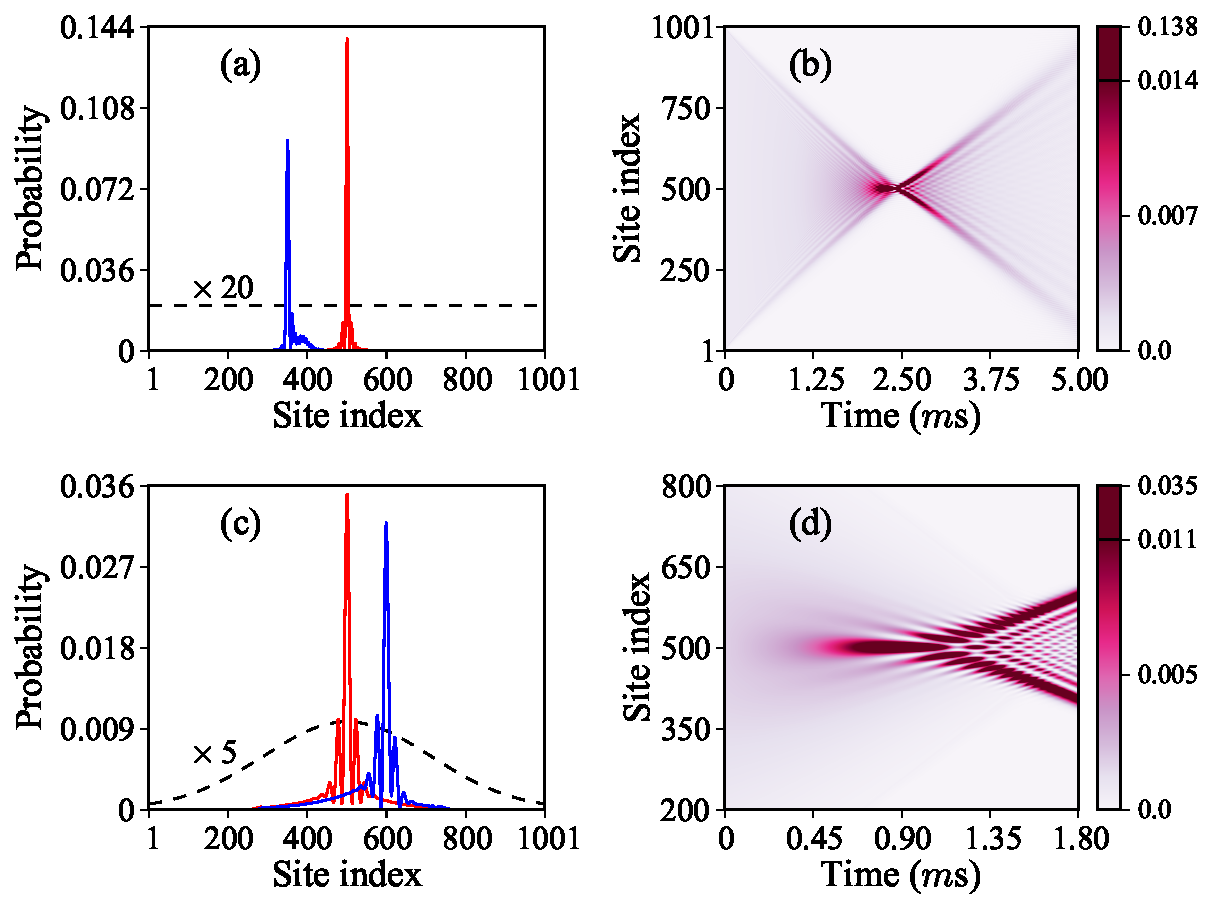
\includegraphics[width=\linewidth]{focusing-1d.pdf}
\caption{ Focusing of a completely delocalized collective
excitation (panels a and b) and a broad Gaussian wave packet of
Frenkel excitons (panels c and d) in a one-dimensional array using the quadratic phase
transformations at $t=0$ as described in text. In panels (b) and (d),
the excitation probability distribution is displayed by color.
The dashed lines
show the initial distribution magnified by 20 and 5 respectively
in (a) and (c). The solid curves in panels (a) and (c) correspond
to two different phase transformations focusing the same wave
packet onto different parts of the array.  The calculations are
performed with the same parameters $\alpha$, $a$, and $\Delta
E_{e-g}$ as in Figure \ref{momentum-kick}. The results are computed
with all couplings accounted for. }\label{focusing-1d}
\end{figure}
%%%%%%%%%%%%%%%%%%%%%%%%%%%%%%%%%%%%%%%%%%%%%%%%%%%%%%%%%%%%%%%%

The focusing scheme demonstrated above can be generalized to  systems of higher
dimensionality. To illustrate this, we repeated the calculations
presented in Figures \ref{focusing-1d} (c) and \ref{focusing-1d} (d) for
a delocalized excitation placed in a square 2D lattice with an external
potential that modulates the phase as a function of both $x$ and
$y$. \Autoref{focusing-2d} shows the focusing of an initially broad wave packet
onto different parts of a 2D lattice induced by the quadratic
phase transformation $\Phi(x,y) = \Phi_0[ (n_x - n_{x_0})^2 + (n_y- n_{y_0})^2]$, 
where $n_x$ and $n_y$ are the lattice site indices along the $x$ and $y$ directions. 
The calculations include all long-range couplings as in \autoref{focusing-1d}. The comparison of \autoref{focusing-1d} and \autoref{focusing-2d} illustrates that the 
focussing efficiency in 2D is greater. The results also demonstrate that the delocalized excitations can be effectively focused on different parts of the lattice simply by varying the reference site $(n_{x_0}, n_{y_0})$ in the phase transformation. 
%Multiple phase kicks of varying profiles separated by periods of free evolution may enable arbitrary shaping of the excitonic wave packet in the coordinate and $k$-spaces.

%%%%%%%%%%%%%%%%%%%%%%%%%%%%%%%%%%%%%%%%%%%%%%%%%%%%%%%%%%%%%%%%%%%%%%%%%%%%%%%%%
\begin{figure}[htbp]
\centering
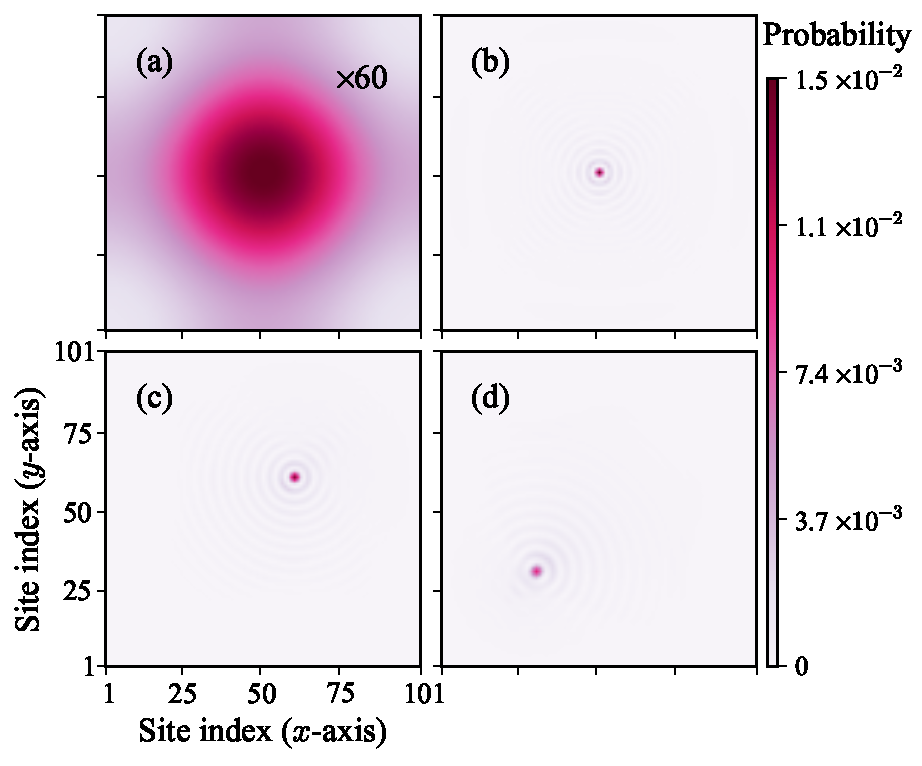
\includegraphics[width=\linewidth]{focusing-2d.pdf}
\caption{Focusing of a delocalized excitation in a 2D array shown
at $t=0$ in panel (a) onto different parts of the lattice (panels
b--d). For better visualization, the probability  distribution in panel (a) is magnified by a factor of 60. The calculations are performed with
the same parameters $\alpha$, $a$, and $\Delta E_{e-g}$ as in
Figure \ref{momentum-kick} and the quadratic phase transformation
at $t=0$.
 }\label{focusing-2d}
\end{figure}
%%%%%%%%%%%%%%%%%%%%%%%%%%%%%%%%%%%%%%%%%%%%%%%%%%%%%%%%%%%%%%%%%%%%%%%%%%%%%%%%%%%


%\section{Controlled excitations of ultracold atoms and molecules}
\section{ Experimental feasibility of phase transformation}
\label{sec:excitationAtomMolecule}

In  \autoref{sec:phaseKicking}  and \autoref{sec:focusing}, we have discussed the idea of phase kicking and its
 application in focusing delocalized excitations, but we were mainly concerned with the theoretical perspective. So in 
this section, we focus on the experimental feasibility and show
the techniques proposed in \autoref{sec:phaseKicking}  and \autoref{sec:focusing}  can be realized with ultracold atoms or molecules trapped in an
optical lattice  with one particle per lattice site \cite{atom-mott1, atom-mott2, atom-mott3, Ye-arrays-PRL12}.
There are three general requirements that must be satisfied:

\begin{itemize}
\item
 (i) The time required for a  phase transformation must
be shorter than the spontaneous decay time of the excited
state.

\item
 (ii) The overall coherence of the system  must be preserved
on the time scale of the excitonic evolution in the entire array, set by $K\hbar/\alpha$, where $K$
 is the number of monomers participating in the dynamics of the collective excitation.

\item
(iii) The lattice constant must be large enough to allow considerable variation of the external
 perturbation from site to site.

%
\end{itemize}

Optical lattices offer long coherence times ($> 1$ sec) and large lattice constants ($>400$ nm)
 \cite{optical-lattice-review}. The lifetime of the
collective excitations depends on the internal states
 of the particles used in the experiment and the momentum distribution of the excitonic states in the wave packet
(\ref{k-rep}). In the following two subsections, we discuss the case of ultracold atoms and the case of ultracold molecules separately. 

\subsection{Collective excitation of ultracold atoms}
\label{sec:excitationAtoms}

For ultracold alkali metal atoms in an optical lattice, an optical excitation may generate collective states (\ref{basis}),
as discussed in Ref. \cite{electronic-exciton1, electronic-exciton2}.
The lifetime of these excited states is limited by the spontaneous emission of the electronically excited atoms and is
in the range of 10 - 30 ns.
However, the collective excited states can be protected from spontaneous emission if the wave vector range populated by excitons in the wave packet (\ref{k-rep}) is
%sufficiently far from zero \cite{cone-matter-papers}. Due to momentum conservation,
outside of the so-called light cone, so that $k >\Delta E_{e-g}/\hbar c$.  
The number of $k$-states in the bright and dark regions depends on the relation between the wavelength of the 
excitation $\lambda_0 = 2\pi c \hbar / \Delta E_{e-g} $ and the lattice constant, with bright states appearing at $k < k_* = 2\pi / \lambda_0$, and dark
states at $k_* < k < \pi/a$. For Frenkel excitons originating from electronic transitions in solid-state crystals, $\lambda_0 \gg a$ and $k_*
\approx 0$. For atoms trapped in optical lattices, the typical values of $\lambda_0 \sim 2a$, and the dark region may be narrow. 
 In an ideal infinite system these states have infinitely long radiative lifetimes, as there is no free-space 
photon they can emit, assuming the conservation of both energy and momentum \cite{electronic-exciton1, 
electronic-exciton2, agranovich1966, agranovich}.
In finite and/or disordered systems, the emission of photons may occur at the array boundaries or due to perturbations 
breaking the translational symmetry. In this case, the time scale for spontaneous decay must depend on 
the size of the system (i.e. the probability of the excitation to reach the array boundary) and the disorder potential 
breaking the translational symmetry.  

 %Due to the same conservation laws,
%single-photon excitation of atomic ensembles always generates excitons with $k \approx 0$.
Once collective excited states are created, the phase-kicking technique introduced in  \autoref{sec:phaseKicking}, 
if implemented on a time scale faster than the radiative lifetime of a single atom, 
can be used to shift the excited states in the wave vector space
away from the light cone (cf. Figure 1) and thus protect the excited states from fast spontaneous decay. This phase transformation can be induced by a pulse of an off-resonant laser field $\mathcal{E}_{AC}$,
detuned from the  $e \leftrightarrow g$ resonance by the value  $\delta\omega$, leading to the
AC Stark shift {(see e.g. Ref.\cite{focusing-books-1})}
\begin{equation}
\Delta E_{AC} =  \mathcal{E}_{AC}^2 \frac{V_{eg}^2}{4 \delta \omega} \ ,
\end{equation}
where $V_{eg}$ is the matrix element of the dipole-induced transition.   By choosing $ V_{eg}= 1$ a.u.,
$\delta \omega = 3 V_{eg}$, and the laser intensity $I = 5\times10^{10}$ W/cm$^2$, we obtain that the shift
 $\phi = \D E_{AC} \times T_{\rm pulse} = \pi $ can be achieved in less than 1 ns. 
%{This shift brings a wave packet initially centered at $k=0$ to the ``dark" edge of the Brillouin zone, where the dispersion of excitons is still quadratic and all the focusing schemes discussed in Section 3 can be applied. 
Another phase transformation can bring the excited state back to the light cone region, where it can be observed via fast spontaneous emission. 
 The experiments with ultracold atoms have demonstrated  the lattice filling factor reaching 99 \%  \cite{atom-mott1, atom-mott2, atom-mott3}.
 The phase transformations proposed here can be used to stabilize excitonic states in ultracold atomic ensembles against spontaneous emission  
for multiple interesting applications \cite{Zoubi1, Zoubi-review}. 

%\begin{equation}
%\D E_{AC} = \mathcal{E}_{AC}^2 \frac{V_{eg}^2}{\delta\omega^2},
%\end{equation}
%where $V_{eg}$ is the matrix elements of the dipole-induced transition.
%By choosing $\delta\omega = V_{eg}/5$,
%and the laser intensity $I = 10^{10}$ W/cm$^2$, we obtain that the
%shift $\phi = \D E_{AC} \times T_{\rm pulse} = \pi $ can be achieved
%in less than 10 ns.

\subsection{Collective excitation of ultracold molecules}
\label{sec:excitationMolecules}

The spontaneous decay problem can be completely avoided by using rotational excitations in an ensemble of
ultracold polar molecules trapped in an optical lattice.
The rotational states are labeled by the quantum
number of the rotational angular momentum $\bm{J}$ and the
projection $M_J$ of $\bm{J}$ on the space-fixed quantization axis
$Z$. We choose the rotational ground state $|J=0, M_J=0\rangle$ as
$|g\rangle$ and the rotational excited state $|J=1, M_J = 0
\rangle$ as $|e\rangle$. The state $|J=1, M_J = 0 \rangle$ is
degenerate with the states $|J=1, M_J = \pm 1 \rangle$. This
degeneracy can be lifted by applying a homogeneous DC electric
field, making the $|g\rangle$ and $|e\rangle$ states an isolated
two-level system. The molecules in different lattice sites are
coupled by the dipole-dipole interaction $V_{\rm dd}(n-m)$.
The magnitude of
the coupling constant $\alpha(n-m) = \langle e_{n} , g_{m} |
{V}_{\rm dd}(n-m) | g_{n}, e_{m} \rangle$ between molecules with
the dipole moment $1$ Debye separated by 500 nm is on the order of
1 kHz \cite{felipe}. Due to the low value of $\Delta E_{e-g}$, the spontaneous emission time of
rotationally excited molecules  exceeds 1 second.

%\tz{discuss decoherence - coupling to phonons, and spontaneous emission time}

For molecules on an optical lattice, one can implement the phase
kicks by modifying the molecular energy levels with pulsed AC or
DC electric fields. The rotational energy levels for $^1\Sigma$
molecules in a combination of weak AC and DC electric fields are
given by \cite{friedrich-95}
\begin{eqnarray}
E_{J,M_J}  &\approx&  BJ(J+1) +  \frac{\mu^2 \mathcal{E}_{DC}^2
}{2B} G(J,M_J) \nonumber \\
&& - \frac{ \alpha_{\perp}\mathcal{E}_{AC}^2 }{4} + \frac{
(\alpha_{||}-\alpha_{\perp})\mathcal{E}_{AC}^2 }{4}F(J,M_J)
 \label{DressedEnery-Sum}
\end{eqnarray}
%
where $B$ is the rotational constant,  $G(0,0) = -1/3$, $G(1,0) =
1/5$, $F(0,0) = -1/3$, $F(1,0) = -3/5$, $\mathcal{E}_{AC}$ is the
envelope of the quickly oscillating AC field, $\alpha_\|$ and
$\alpha_{\perp}$ are the parallel and perpendicular
polarizabilities and $\mu$ is the permanent dipole moment of the
molecule.

The momentum shift of the exciton wave packets can be achieved by
applying a time-varying DC electric field $\mathcal{E}(t)
=\mathcal{E}_{\ast} + \mathcal{E}(n)\sin^{2}(\pi t/T)$, where
$\mathcal{E}(n)$ is linear with respect to $n$. Assuming that
$\mathcal{E}(n) = (n-n_0) A$ and $\mathcal{E}(n) \ll
\mathcal{E}_{{\ast}}$, and using \autoref{phase} and
\autoref{DressedEnery-Sum}, gives  $\delta = 4 A
\mathcal{E}_{{\ast}} \mu^2 T / 15 \hbar B a$. We have confirmed
this result by a numerical computation showing that for LiCs
molecules in an electric field of $\mathcal{E}_{{\ast}}=1$ kV/cm,
an electric field pulse with $A=7.434\times 10^{-4}$ kV/cm and
$T=1$ $\mu$s results in a kick of $\delta = \pi/2 a$, bringing an
excitonic wave packet from the $k=0$ region to the middle of the
dispersion zone.

An alternative strategy is to use a pulse of an
off-resonance laser field, as for atoms. The phase transformations can be induced
by a Gaussian laser beam with the intensity profile
\begin{equation}
I(r, z) = \frac{I_0}{1+
\frac{z^2}{z_R^2}}\exp\left[-\frac{2r^2}{w_0^2\left (1+
\frac{z^2}{z_R^2}\right) }\right] \ ,
\label{gaussian-intensity-profile}
\end{equation}
where $I_0$ is the light intensity at the beam center, $r$ is the
radial distance from the center axis of the beam, $z$ is the axial
distance from the beam center,  $z_R=\pi w_0{\color{red}^2}/\lambda$ is
Rayleigh range, $w_0$ is the beam waist and $\lambda$ is the wavelength.
With the 1D molecular array arranged along the $z$-axis, the laser field intensity
can be made to vary nearly linearly along the array,
\begin{equation}
I(r=na, z=0; t) \approx [I_{c} + n I_1 ] \, \sin^{2}(\pi t/T) \; \;\; (0 < t <
T) \ , \label{intensity-varying}
\end{equation}
where $I_{c}$ is the intensity at the center of the wave packet.
This can be achieved if $z_0 = z_R/\sqrt{3}$ and ${\sigma}_x^{(2d)}
a\lesssim 0.5 z_R$, where $z_0$ is the distance between
the center of the wave packet and the beam center, and ${\sigma}_x^{(2d)}$ is the width (in the coordinate representation) of the two-dimensional wave packet. Using \autoref{phase}, \autoref{DressedEnery-Sum} and (\ref{gaussian-intensity-profile}), we estimate the momentum kick by such a pulse as $
%\begin{equation}
\delta = -\sqrt{3}T I_{0} (\alpha_{\|}-\alpha_\perp) / 80 z_R
%~. \label{Kick-AC}
%\end{equation}
$.
The results presented in Figure 1 were obtained for a 1D array of LiCs molecules on an optical lattice with $a=400$ nm and the external perturbation
given by the laser field pulse (\ref{intensity-varying}) with parameters $I_c$ and $I_1$ derived from  \autoref{gaussian-intensity-profile} with $z_0 = 45\; \mu$m and
$z_R=73.8\; \mu$m. The numerical results deviate from the analytical prediction for $\delta$ by less than 7 \%.

The Gaussian intensity profile (\ref{gaussian-intensity-profile}) can be used also to implement the quadratic phase transformations needed for focusing of collective excitations. %The quadratic phase transformations needed for focusing of collective excitations can also be implemented by a laser beam with a Gaussian intensity profile.
To achieve this, a 2D molecular array must be arranged in the $z=0$ plane,
with the  $x$-axis defined to be along the polarization direction of a linearly polarized field.
If the dimension of the molecular array is smaller than one third of the
beam waist, the Gaussian intensity profile in
\autoref{gaussian-intensity-profile} can be approximated
%\tb{``, to better than 90 \%," -- let's cancel it? This may depend on parameters of the system...} 
by
\begin{equation}
I(r=na, z=0; t) \approx I_{0}\left[1- \frac{2(n_x^2 +
n_y^2)a^2}{w_0^2}\right]. 
\label{quadratic-profile}
\end{equation}
This is a concave quadratic intensity
profile which can be used to focus a wave packet  in a system with negative couplings $\alpha$ (see \autoref{sec:focusing}).



\section{Control of energy transfer in dipolar systems}
\label{sec:controlEnergyTransfer}

Dipolar interactions play a central role in the study of long-range interaction effects using ultracold systems \cite{our-njp-review}.
While, in general, the coupling constant $\alpha$ in \autoref{ham} can be determined by a variety of interactions, the dominant contribution to $\alpha$ for atoms and molecules on an optical lattice is determined by the matrix elements of the dipole - dipole interaction. It is therefore particularly relevant to discuss the specifics of energy transfer in systems with dipolar interactions. 

The dipolar interactions are long-range and anisotropic. This long-range character
manifests itself in the modification of the exciton dispersion (\ref{Eexc}). While \autoref{Eexc} is valid for a system 
with nearest neighbour couplings only, higher-order couplings in the case of $\alpha(n-m) \propto 1/ |n-m|^3$ 
modify the exciton dispersion leading to a cosine-like, 
but non-analytic dispersion relation, both in 1D  and 2D. 
To investigate the effect of this nonanalyticity in dispersion curve, we have performed a series of calculations with the long-range couplings neglected 
after a certain lattice site separation $n-m$ for the 1D system. The results become  converged (to within 0.2 \%) when
 each molecule is directly coupled with 20 nearest molecules. While the calculations with only the nearest neighbor
 couplings are in good agreement  with the analytical predictions given by \autoref{focus-time} and \autoref{x-focusing-Gauss}, the full calculations reveal that long-range 
couplings somewhat decrease the focusing efficiency. The long-range couplings also decrease the focusing time, 
by up to a factor of 2. The dynamics of collective excitations leads to interference oscillation patterns clearly 
visible in panels a and c of Figure \ref{focusing-1d}. These oscillations are much less pronounced when all but nearest
 neighbor couplings are omitted. The numerical results of Figures 1 - 3 are particularly important
 because they demonstrate that the phase transformations introduced in the present work are effective  for 
systems with dipolar interactions. 


The anisotropy of the dipolar interactions can be exploited for controlling energy transfer in dipolar systems by varying the {\it orientation} of a dressing external DC electric field. 
For example,  for polar molecules on an optical lattice,  
the matrix elements  $\alpha(n-m) = \langle e_{n} , g_{m} | {V}_{\rm dd}(n-m) | g_{n}, e_{m} \rangle$ depend not only on the choice of
 the states $|g\rangle$ and $|e\rangle$, but also on the magnitude and orientation of an external dc electric field
\cite{biexcitons, felipe}. Since the value of $\alpha$ determines the exciton dispersion (\ref{Eexc}),
 the exciton properties can be controlled by varying the angle $\theta$ between the intermolecular axis
and the applied DC field. This is illustrated in Figure 4. 

The calculations presented in Figure \ref{control-exciton} are for a 1D array of LiCs molecules in a lattice with  $a=400$ nm.
As before, $|g\rangle$ is the absolute ground state of the molecule and $|e\rangle$ is the rotationally excited state
 that adiabatically correlates
with the rotational state $|J=1, M_J = 0 \rangle$ in the limit of vanishing electric field. 
The upper panel of Figure 4
shows that the angle $\theta$ between the electric field vector and the molecular array axis
determines the sign and magnitude of $\alpha$, and therefore the shape of the dispersion
curve. This enables
control over the sign and magnitude of the group velocity of an
excitonic wave packet containing contributions with $k\neq 0$. Dynamically tuning $\theta$,
one can propagate a localized excitation to different parts of the
lattice, as shown in Figure \ref{control-exciton} (b).

In a 2D lattice, the intermolecular interactions depend on an additional azimuthal angle $\phi$ that describes
 the rotation of the electric field axis around the axis perpendicular to the lattice. The numerical calculations 
presented in Figure \ref{control-2d-wavepacket} show that the energy flow in two dimensions can be  
controlled by varying both $\theta$ and $\phi$. 
In addition to the phase transformation discussed earlier, this allows for a dynamical energy transfer in quantum 
many-body systems with anisotropic interparticle interactions.



%%%%%%%%%%%%%%%%%%%%%%%%%%%%%%%%%%%%%%%%%%%%%%%%%%%%%%%%%
\begin{figure}[htbp]
\centering
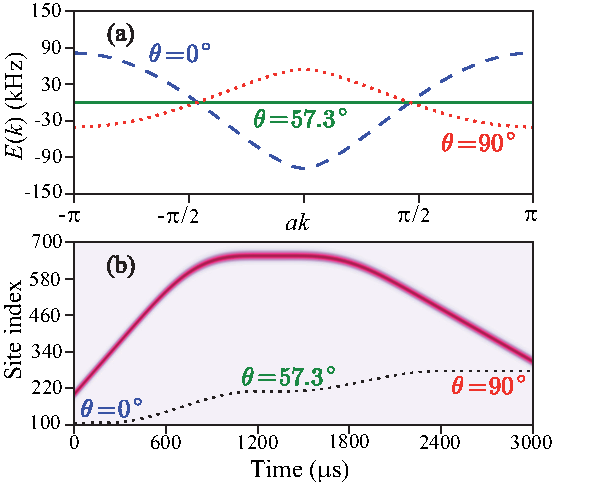
\includegraphics[width=\linewidth]{control-exciton.pdf}
\caption{ Control of excitation transfer in a 1D many-body system with dipolar interactions by varying the 
direction of an external electric field.
Panel (a): Exciton dispersion curves for a 1D
ensemble  of diatomic molecules on an optical lattice for
different angles $\theta$ between the direction of the external DC
electric field and the axis of the molecular array.  In 1D, the coupling $\alpha\propto (1/3 - \cos^2\theta)$.  Panel (b):
Propagation of a wave packet centered at $ak =-\pi/3$ controlled
by tuning the electric field direction. Thin dotted line depicts
the corresponding angle variations with time. The brightness
of color corresponds to the probability of the excitation. }
\label{control-exciton}
\end{figure}
%%%%%%%%%%%%%%%%%%%%%%%%%%%%%%%%%%%%%%%%%%%%%%%%%%%%%%

%%%%%%%%%%%%%%%%%%%%%%%%%%%%%%%%%%%%%%%%%%%%%%%%%%%%%%%%%
\begin{figure}[htbp]
\centering
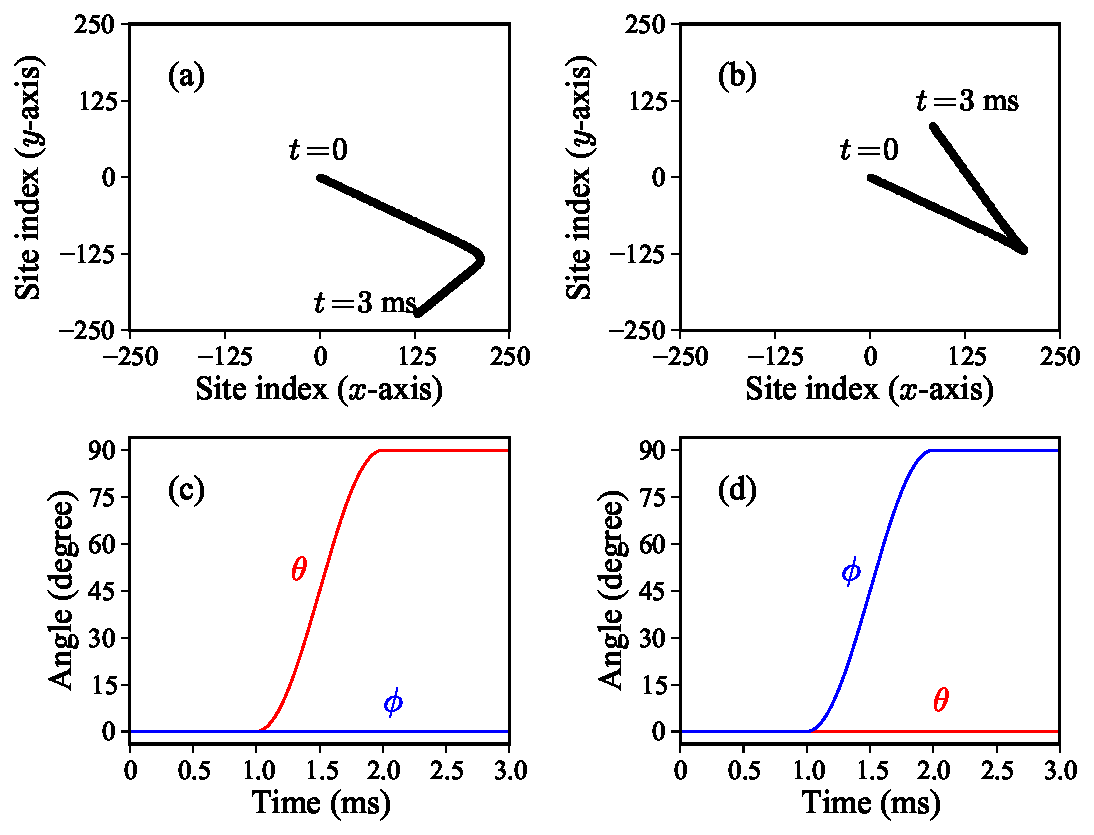
\includegraphics[width=\linewidth]{control-2d-wavepacket.pdf}
\caption{ Control of excitation transfer in a 2D many-body system with dipolar interactions by varying the 
direction of an external electric field.
Panels (a) and (b) show the trajectories of the center of an exciton wave packet in a 2D lattice during
 the time from 0 to 3 ms; Panels (c) and (d) represent the changing of the dressing DC field orientation $(\theta, \phi)$ associated with (a) and
(b) respectively. The initial wave packet is a 2D Gaussian distribution centered around $ak_x=ak_y=\pi/2$ and has a width of $\sim$60 lattice sites in coordinate space. The magnitude of the DC field is fixed to
6 kV/cm while its direction is changing. The calculations are done for a 2D array of  LiCs molecules in a lattice with
$a=400$ nm.
 }
\label{control-2d-wavepacket}
\end{figure}
%%%%%%%%%%%%%%%%%%%%%%%%%%%%%%%%%%%%%%%%%%%%%%%%%%%%%%

\section{Energy transfer in the presence of vacancies}
\label{sec:energyTransferVacancy}

While experiments with ultracold atoms have produced states with one atom per lattice site with  99\%  fidelity \cite{atom-mott1, atom-mott2, atom-mott3},
the latest experiments with molecules yield lattice-site populations about  10\% \cite{Ye-arrays-PRL12}.
Multiple experiments are currently underway to  trap polar molecules on an optical lattice with close to the full population of the lattice.
However, lattice vacancies may be unavoidable in the best experiments. In this section, we examine the effect of vacancies on the possibility of focusing collective excitations
to a desired region of the lattice by the phase transformations discussed in \autoref{sec:focusing}. For concreteness, we perform calculations for the system described in \autoref{sec:excitationAtomMolecule},
namely a 2D array of LiCs molecules on a square optical lattice with $a=400$ nm.



To explore the effect of vacancy-induced interactions, we performed simulations for
different vacancy numbers using the same parameters for molecule-field and inter-molecular interactions as
in the calculations presented in Figure \ref{focusing-2d}b. For each vacancy concentration, we carried out 48
calculations with random distributions of empty lattice sites. The quadratic phase transformations are applied,
as described in \autoref{sec:focusing}, in order to focus the collective excitation at time $t_{\ast}$ to
the molecule in the middle of the 2D array.

Vacancies disturb the translational symmetry of the system and produce an effective disorder potential that tends to
localize collective excitations \cite{perez-rios2010}.
 Because the natural time evolution of the wave packet in a disorder potential may lead to enhancement of the probability in certain
regions of the lattice, it is necessary to distinguish the effect of the vacancy-induced localization and the effect of the focusing phase
transformation. To quantify these two effects, we define two factors:
the enhancement of the probability at the target molecule with respect to the initial value,
\begin{equation}
\eta = \frac{p' (t=t_{\ast})}{p(t=0)},
\label{eta}
\end{equation}
and the ratio of the probability to find the excitation on the target molecule with ($p'$) and without ($p$) the focusing
phase transformation,
\begin{equation}
\chi = \frac{p' (t=t_{{\ast}})}{p (t=t_{ {\ast}})}.
\end{equation}
The time $t_*$ is the focusing time found numerically for the corresponding vacancy-free system.
 The quantity $\eta$ illustrates the actual enhancement of the probability to focus a collective excitation,
while the quantity $\chi$ illustrates the effect of the focusing phase transformation.
Figure 6 presents the values of $\eta$ and $\chi$ as functions of the vacancy concentration.
It illustrates two important observations. First, the disorder potential with vacancy concentrations $> 20$ \%
renders the phase transformation ineffective. In the presence of strong disorder, the dynamics of the system is entirely
determined by the disorder potential and the energy transfer becomes highly inefficient (however, see \autoref{sec:focusingStrongDisorder}). On the other hand, vacancy
concentrations of less than 10 \% appear to have little effect on the efficacy of the focusing phase transformation.

Our calculations indicate that the focusing time may be somewhat modified by the disorder potential, even if the
 concentration of vacancies is less than 10 \%.  Figure 7 depicts the excitation wave functions
 at the time of the maximal enhancement on the target molecule, chosen as molecule (71,71).  Figure \ref{focusing-with-vacancy} shows that
despite the presence of multiple vacancies, the focusing transformation enhances the probability to find the
excitation on the target molecule by 16 times.


% As you can see from Figure \ref{enhancement-vs-vacancy}, the enhancement factors decrease exponentially as vacancy percentage increases, but still a relatively good focusing can be achieved with 10\% of vacancies.

\begin{figure}[htbp]
\centering
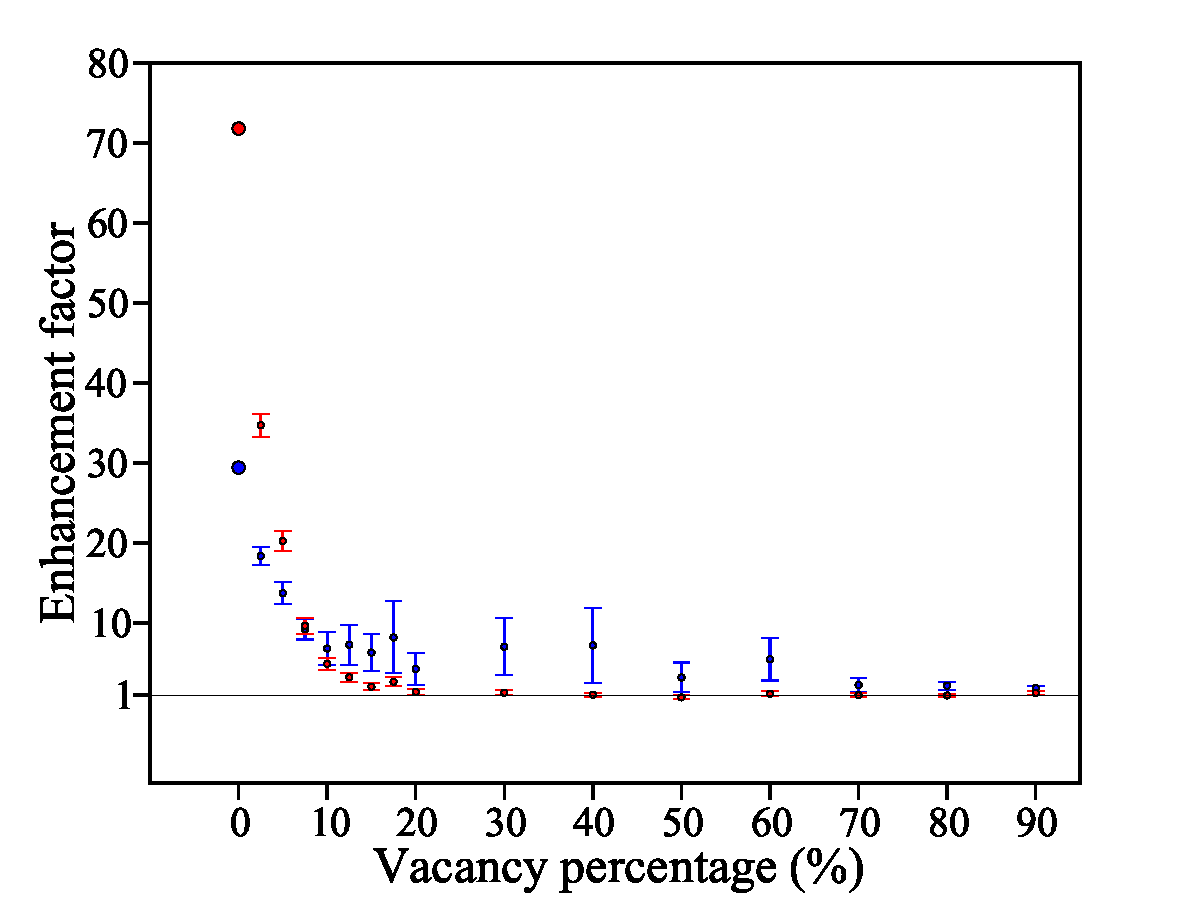
\includegraphics[width=\linewidth]{enhancement-vs-vacancy.pdf}
\caption{ Enhancement factors $\eta$ (red symbols) and
$\chi$ (blue symbols) as functions of vacancy percentage in a 2D lattices. See text
for the definitions of $\eta$ and $\chi$. The error bars are for 95\% of confidence interval. 
} 
\label{enhancement-vs-vacancy}
\end{figure}

%Due to the presence of vacancies in optical lattices, the focusing time $T_{\tiny \mbox{target}}$ for a full lattices would not be the focusing time for a partial lattices. So it is a little unfair to use  $T_{\tiny \mbox{target}}$ as the time for comparison in Figure \ref{enhancement-vs-vacancy} and actually the focusing, as shown in Figure \ref{focusing-with-vacancy},  can be better if the real focusing time is chosen.



\begin{figure}[htbp]
\centering
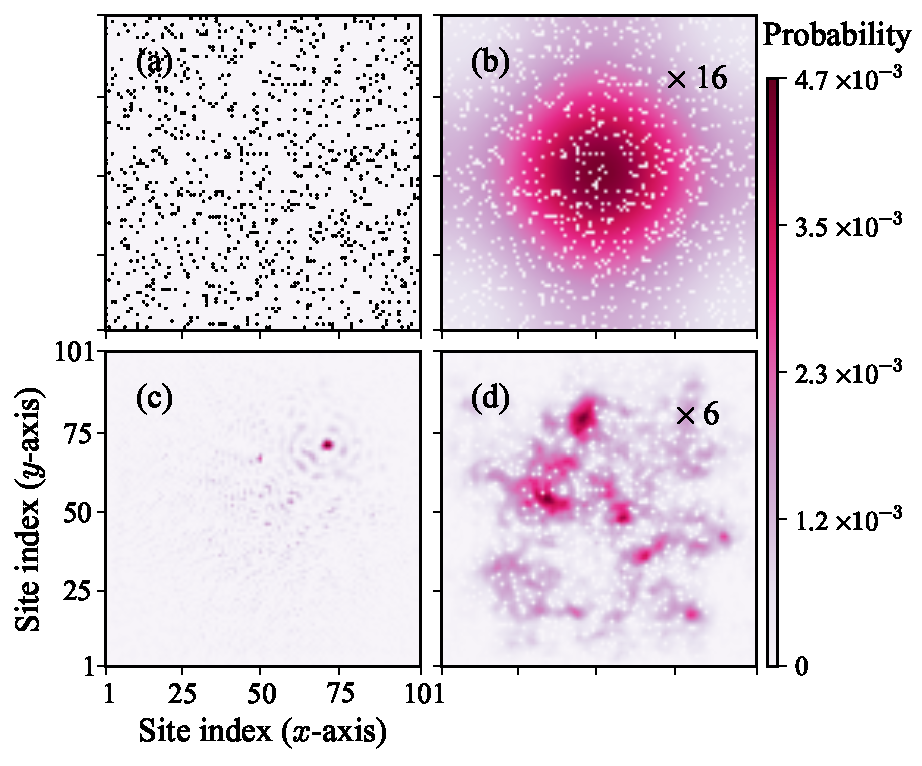
\includegraphics[width=\linewidth]{focusing-with-vacancy.pdf}
\caption{  Time snapshots of a collective excitation in a 2D
array with a vacancy concentration of 10 \%  (a) The distribution of the vacant sites; (b) The initial probability distribution of the excited state; (c) The probability distribution of the excitation at the
focusing time when the focusing scheme is applied. The focusing
time is  found numerically as  the time when the probability at the target
molecule (71, 71) reaches maximum  for a given phase transformation. (d) The probability
distribution of the wave function at the focusing time when the
focusing scheme is not applied. The calculations are performed
with the same parameters as in Figure \ref{focusing-2d}. The
probabilities in (b) and (d) are magnified by 16 and 6
respectively. } \label{focusing-with-vacancy}
\end{figure}

\section{Focusing in the presence of strong disorder}
\label{sec:focusingStrongDisorder}

%\tb{We need to cite something about t-matrix focusing. Zhenia, could you insert citations into the following paragraphs? }

Although the focusing method demonstrated in \autoref{sec:focusing} and \autoref{sec:energyTransferVacancy} appears to be robust in the presence of a disorder potential induced by a small concentration of vacancies, it is important for practical applications to also consider controlled energy transfer in quantum arrays under a strong disorder potential. To consider focusing in a strongly disordered system, 
we employ an analogy with the {``transfer
matrix'' methods for focusing of a collimated light beam in opaque
medium \cite{opaque-1, Gigan-TMeasure-PRL10, Mosk-NPhot10, Cizmar-NPhot10, Silberberg-11, Chatel-Focusing-11, Lagendijk-Focusing-11, zhenia-11, cui-11, kim-11}}.


In optics, a collimated laser beam passing through an opaque medium results in a random
pattern of speckles arising from random scattering of light inside the medium
\cite{RandomWave-books}. Likewise, the random distribution of empty sites in an optical lattice with molecules 
scatters the exciton wavepackets, resulting in a completely random excited state. 
However, in optics, the randomness of the scattering centers inside the opaque medium can be compensated for by
shaping the incident wavefront with a spatial light modulator such
that the contributions from various parts of the medium can add
constructively upon exit from the medium, producing a focus. 
We suggest that the same can be achieved with a many-body system on a lattice by 
separating the entire lattice into multiple blocks and applying proper phase transformations
to those individual blocks. 



%Here we consider an \tz{initial state} \tb{[I like this $|i\rangle$-notation, but probably we should use instead $c_i(t=0) |e_i\rangle \prod_{j\neq i} |g_j\rangle$ to simplify the comparison with Eq.(2)?]}
%plane-wave like initial state with the same probability for each
%occupied site and zero probability for each vacancy site:
%

The initial state for an ensemble of molecules on a lattice with multiple vacancies can be written as 
\begin{equation}
|\psi(t=0)\rangle = \sum_{i}c_i(t=0)|i\rangle \ , \label{planewave-initial}
\end{equation}
where 
\begin{eqnarray}
| i \rangle = |e_i\rangle \prod_{j\neq i} |g_j\rangle
\end{eqnarray}
and the indexes $i$ and $j$ run over all occupied sites. After a long evolution time $T$, the probability amplitude for the excitation to reside on a particular target molecule is given by  
\begin{equation}
c_{o}(T) = \sum_{i} U_{o, i}(T)c_i(t=0) \equiv \sum_i c_{oi}(T), 
\label{site-contribution}
\end{equation}
where $U_{o,i}(t) = \langle o| \exp[-iH_{\rm exc}t] | i \rangle$ is a matrix element of the time evolution operator.
%
{In a disordered system, the transfer coefficients $U_{o, i}$
are not a-priori known and depend on the
disorder potential. The {phasors} $c_{oi}(T)$ have quasi-random
amplitudes and phases. While the amplitude of each phasor cannot be controlled experimentally, 
their phases are controllable via the phases of the coefficients $c_i$ at $t=0$, which can be tuned using the phase-kicking
transformations introduced above.} To achieve the highest probability
at the target molecule, it is necessary to ensure that the contribution
$c_{oi}=U_{o, i}(T)c_i(t=0)$ from every site $i$ has the same
phase so that they add up constructively.

In a practical implementation, it may be difficult to control the phase of each molecule in each
individual site. It may be more desirable to work with blocks of several lattice sites. Assuming that the entire array of molecules 
can be divided into $M$ blocks, each containing many molecules, and that the blocks can be perturbed individually, the excitation probability amplitude at the target molecule at time $T$ is 
%\tz{Let us divide the whole array into $N$ blocks (``channels''), each containing many molecules, in such a way that it is possible to apply an overall phase to molecules in one block without perturbing the others. The excitation at the target molecule at time $T$ is}
%
\begin{equation} c_{o}(T) =  \sum_{\gamma=1}^M c_{\gamma}(T)
\label{blocks-contribution}
\end{equation}
%
where
%
\begin{equation} c_\gamma(T) \equiv |c_\gamma| e^{i\phi_\gamma}= \sum_{i\in
 \gamma} U_{o, i}(T)c_i(t=0) \ .
\label{inblock-contribution}
\end{equation}
%
%
%So we work with sub-blocks of lattice sites and Eq.v(\ref{site-contribution}) becomes
%\begin{equation}
%c_{o}(T) = \sum_{M} \tilde{U}_{o, M}(T)b_M(t=0) \ , \label{block-contribution}
%\end{equation}
%where $M$ is the index for the sub-blocks, and $b_M$ is the vector whose components are coefficients $c_j$'s of sites insidethe sub-block $M$:
%\begin{equation}
%b_M(0) =\left(
%   \begin{array}{c}
%   c_1^{M}(0) \\
%   c_2^{M}(0) \\
%  \cdot \\
%  \cdot \\
%  \cdot \\
%  c_n^{M}(0)
%   \end{array}
%\right) \ , \label{block-coeff}
%\end{equation}
%tz{rewrite in conventional math notations from here} and the element $\tilde{U}_{o, M}$ of the new time evolution matrix  is related to $U_{o, i}$ by the following equation:
%\begin{equation}
%\tilde{U}_{o, M} = \left( U_{o, j}, U_{o, k}, \cdots, U_{o, r}\right) \ , \label {block-evolution0}
%\end{equation}
%where sites $j, k, \cdots, r$ belong to the sub-block $M$. We can rewrite Eq. (\ref{block-evolution0}) as
%\begin{equation}
%\tilde{U}_{o, M} = \left( U_{o, 1}^M, U_{o, 2}^M, \cdots, U_{o, n}^M\right) \ , \label {block-evolution}
%\end{equation}
%to emphasize that all the components are related to occupied sites in sub-block $M$.Substituting Eq. (\ref{block-coeff}) and (\ref{block-evolution}) into Eq. (\ref{block-contribution}), we have
%\begin{equation}
%c_{o}(T) = \sum_{M} c_M(T) \ ,
%\end{equation}
%where each block contributes
%\begin{equation}
%c_M(T) = \sum_{j=1}^{n} U_{o, j}^M (T) c_j^{M}(0) = |c_M| \exp(i
%\phi_{M}) \ . \label{cM}
%\end{equation}
This equation implies that the contributions
from different blocks can be made to interfere constructively by adding
 a phase $\exp(-i \phi_{\gamma})$ to each occupied site in block
 $\gamma$. For $M$ blocks in the array and quasi-random evolution matrix, simply setting all the phases equal
 must lead to $\sim M$-fold increase of the excitation probability at the target molecule, as compared to
 a sum of $M$ quasi-random phasors in \autoref{blocks-contribution} \cite{opaque-1}.

Similarly to optics, the phases $-\phi_\gamma$ which must be added in each block, can be found experimentally provided
that the same (or similar) realization of disorder persists in a series of
trials. A straightforward optimization would scan through the
strengths of  phase kicks applied to different blocks. In each
experiment one would measure the excitation probability at the
target molecule $|c_o(T)|^2$, e.g. via resonance fluorescence from
the target molecule at the end of the experiment. More
sophisticated optimization techniques, aimed at fast focusing
multi-frequency light in optical systems, are currently under
rapid development \cite{Gigan-TMeasure-PRL10, Mosk-NPhot10, Cizmar-NPhot10, Silberberg-11, Chatel-Focusing-11, Lagendijk-Focusing-11, zhenia-11, cui-11, kim-11}.


%\tz{However, numerically we find the phases $\phi_M$ in a faster way.{ CONSULT WITH PING WHETHER WHAT IS BELOW IS EXACTLY WHAT HE DID IN THE CALCULATION}} 

For a proof-of-principle calculation, we consider a 2D lattice of size 101$\times$101 with 60\% of sites vacant and each non-vacant site occupied by a single LiCs molecule. 
Due to time reversibility of the time
evolution operator $U(T)$, 
%the phase $\exp(-i \phi_{M})$ can be obtained as follows:
\begin{equation}
|c_\gamma | \exp(-i \phi_{\gamma}) = \left[ \sum_{j=1}^{n} U_{o, j}^\gamma (T) c_j^{\gamma}(0)\right]^* 
=\left[ \sum_{j=1}^{n} U_{j, o}^\gamma (-T) c_j^{\gamma}(0)\right]^* \ .
\end{equation}
The matrix element $U_{j, o}^\gamma (-T)$ can be
calculated by performing a backward time propagation starting from a
local excitation at site ``$o$'' and calculating the coefficient
$c_j(t)$ at time $-T$. Alternatively, one can propagate the evolution equations forward in time, finding $c_j(T)$: 
Since the Hamiltonian (1) is real, its eigenfunctions are real, and the evolution matrix $U$ is symmetric, $U_{o, j} = U_{j, o}$. Thus we find
\begin{equation}
c_j(T) = \sum_{i}U_{j, i}^\gamma (T) c_i(0) = U_{j, o}^\gamma (T) \ ,
\end{equation}
since $c_{o}(0) = 1$ and all other coefficients are zero. For a completely delocalized initial state, we assume that all coefficients
in auto\ref{planewave-initial} are equal, so that  the phases $\phi_\gamma$ required for
block $\gamma$ are
\begin{equation}
 |c_\gamma|\exp(- i \phi_{\gamma})  = \left[ \sum_{j}  c_j(T) \right]^* \ , \label{phase-applied}
\end{equation}
where the index $j$ runs over all  occupied sites in block $\gamma$.
Figure \ref{t-matrix-focusing} shows that this choice of phases leads to effective focusing of the collective excitation in a strongly disordered system. 

\begin{figure}[htbp]
\centering
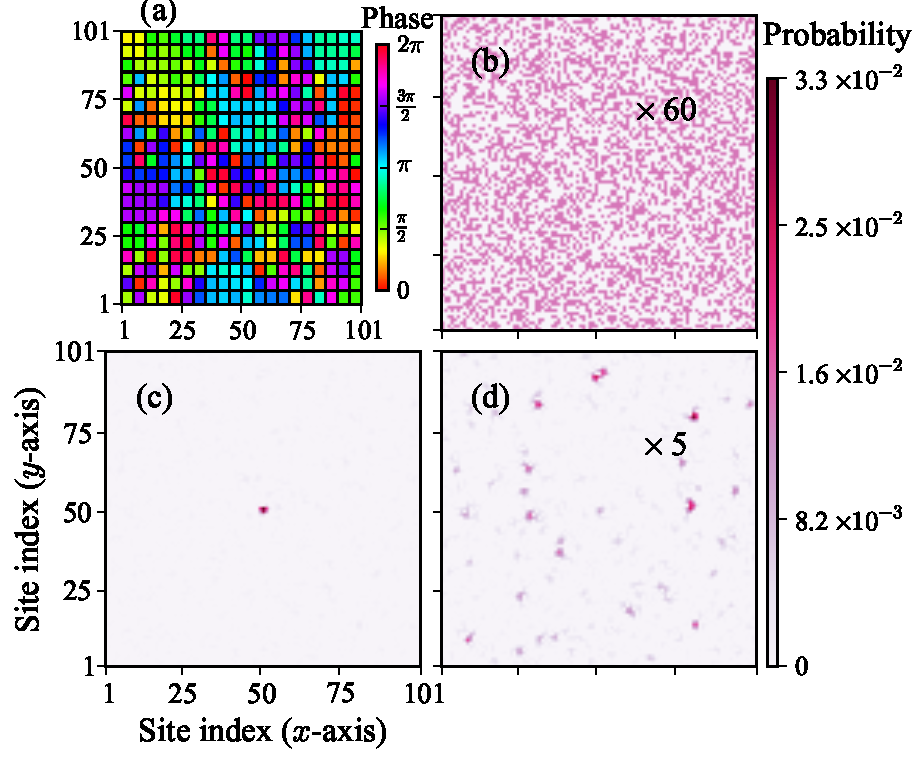
\includegraphics[width=\linewidth]{t-matrix-focusing.pdf}
\caption{  Focusing of a collective excitation in a strongly disordered system with 60\% of lattice sites unoccupied.  Panel (a) shows different phases applied to
different blocks of the lattice before the time evolution.
(b) The initial probability distribution of the excited state. (c) The probability distribution of the excited state at the
focusing time $T = 3$ ms with the phase transformation depicted in panel (a) before the time
evolution. (d) The probability distribution of the excited state at the focusing time $T = 3$ ms with no phase transformation
applied. The calculations are performed
with the same parameters as in Figure \ref{focusing-2d}. The
probabilities in (b) and (d) are magnified by 60 and 5,
respectively. } \label{t-matrix-focusing}
\end{figure}


To illustrate the efficiency of the focussing method described above, we have carried out a series of calculations 
with different vacancy concentrations. For each vacancy concentration, we performed 48 calculations with random
 distributions of empty lattice sites. The phase transformations are calculated individually for each random 
distribution of vacancy sites as described above. The results are shown in Figure \ref{enhancement-vs-vacancy-t-matrix}. 
As can be seen, the transformations proposed above are effective for vacancy concentration $<$ 70\%. At higher 
concentrations of vacancies, the excited states become strongly localized and immobile. The focusing efficiency at
vacancy concentrations 10\% and 20\% appears to be higher than that in the absence of vacancies, which we attribute to the effect of 
the boundaries.
\begin{figure}[htbp]
\centering
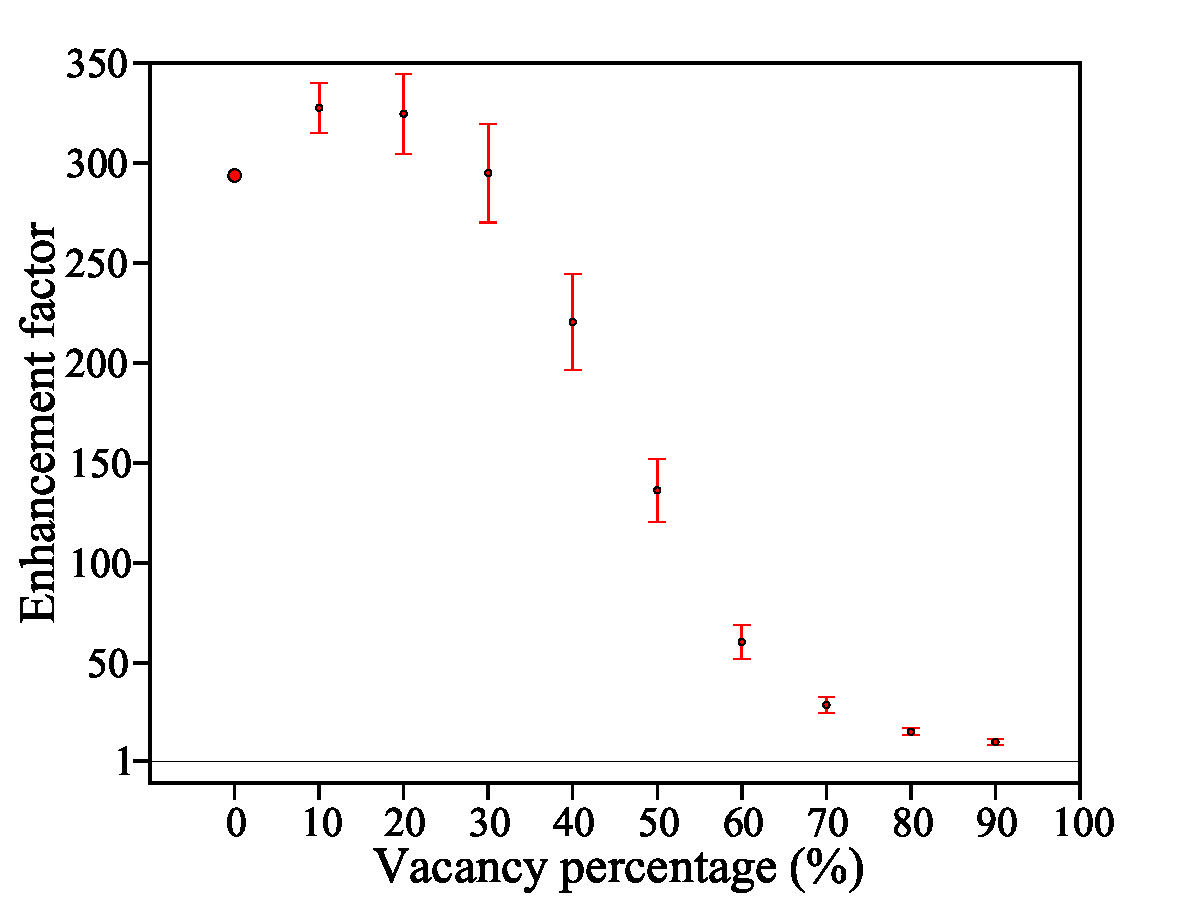
\includegraphics[width=\linewidth]{enhancement-vs-vacancy-t-matrix-other.pdf}
\caption{Efficiency of focusing collective excitations in strongly disordered 2D lattices. The molecular 
array  is divided into 400 blocks as shown in Fig.\ref{t-matrix-focusing}(a). The focusing time $t_*$ is arbitrarily set to 4 ms. For each 
realization of disorder, we use Eq.(\ref{phase-applied}) with $T=t_*$ to find the phase mask applied to different blocks. 
Shown are the enhancement factors $\eta$ (red symbols) defined in Eq.(\ref{eta}), as a function of the vacancy percentage.
 The error bars are for 95\% confidence interval.
%Enhancement factors $\eta$ (red symbols) as a function of vacancy percentage in a 2D lattices. 
%$\eta$ has the same definition as in  Eq. (\ref{eta}) except the time $t_*$ is arbitarily chosen to be 4 ms here. 
% The error bars are for 95\% of confidence interval.
} 
\label{enhancement-vs-vacancy-t-matrix}
\end{figure}

\section{Conclusion}
\label{sec:energyTransferConclusion}

We have proposed a general method for controlling the time evolution of quantum energy transfer in ordered 1D and 2D arrays of coupled monomers.
Any elementary excitation in an aggregate of coupled
monomers can be represented as a coherent superposition of Frenkel
exciton states. We propose shaping the exciton wave
packets using nonadiabatic perturbations that temporarily
modulate the energy levels of the monomers leading to monomer-dependent linear phase transformation and a
displacement of the wave packets in the wave vector representation.
This, combined with the possibility of focusing a collective excitation on a particular part of the lattice by a quadratic phase transformation and with the directed propagation of collective excitations,
allows for control of energy transfer in the lattice. 
An experimental observation of the excitations described here can be achieved by measuring
 site-selective populations of the molecular or atomic states by applying a gradient of an electric field and
 detecting resonant transitions from Stark-shifted levels \cite{demille}.


We have presented numerical calculations for an ensemble of polar molecules trapped on an optical lattice that demonstrate the feasibility of
both momentum-shifting and focusing of collective excitations by applying external laser fields, with parameters that can be easily achieved in the laboratory.
We have also investigated the effect of disorder potential arising from incomplete population of the lattice. Our results show that the phase transformations
 leading to focusing of collective excitations on different regions of a 2D lattice remain effective in the presence of vacancies
with concentrations not exceeding 10 \%. For systems with larger concentrations of vacancies and affected by strong disorder potentials, we propose an alternative procedure based on engineering constructive interference of the wave function contributions arising from difference parts of the lattice. 


The momentum-shifting technique proposed here can be used to protect collective excitations of ultracold atoms from spontaneous emission. 
 The spontaneous decay processes, which in the case of an ordered many-body
system must satisfy both the energy and wave vector conservation rules, can be restricted by shifting the exciton
 wave packets to a region of the dispersion curve, where the wave vector conservation cannot be satisfied.
If performed faster than the spontaneous emission time, such phase transformations should create collective
excitations with much longer lifetimes, which opens a variety of new applications for ultracold atoms on an optical
lattice.




As was proposed by multiple authors \cite{QI-wavepacket1,QI-wavepacket2,QI-wavepacket3,
QI-wavepacket4,QI-wavepacket5,QI-wavepacket6}, molecular wavepackets can be used to 
encode quantum information.  Similarly, collective excitations can be used for quantum memory
\cite{peter-rabl, peter-rabl2}.
Control over excitation transfer is needed for creating networks
of quantum processors where information is transmitted over large
distances with photons and stored in arrays of quantum monomers
via one of the quantum memory protocols \cite{Lvovsky-Qmemories}.
Momentum kicking can be used for wave packet transport within a
single array. Focusing excitonic wave packets would enable local
storage of information, while directed propagation combined with controlled interactions of multiple
excitons \cite{biexcitons} or excitons with lattice impurities
\cite{zoller-atom-transistor} may be used to implement logic
gates. Controlled energy transfer in molecular arrays may also be used
for the study of controlled chemical interactions for a class of
reactions stimulated by energy excitation of the reactants.
Directing  energy  to a particular lattice site containing
two or more reagents can be used to induce a chemical interaction
\cite{pccp}, an inelastic collision or predissociation
\cite{wallis-krems}  with the complete temporal and spatial
control over the reaction process.

Finally, the present work may prove to be important for simulations of open quantum systems. 
We have recently shown \cite{felipe, felipe-arxive-polaron} that
the rotational excitations of ultracold molecules in an optical lattice can,
by a suitable choice of the trapping laser fields, be effectively coupled to lattice phonons.
The exciton - phonon couplings can be tuned from zero to the regime of strong interactions
\cite{felipe, felipe-arxive-polaron}. The possibility of shaping (accelerating, decelerating and focusing)
collective excitations as described in the present work combined with the possibility of coupling these excitations
to the phonon bath opens an exciting prospect of detailed study of controlled energy transfer in the presence of a
controllable environment. Of particular interest would be to study the effect of the transition from a weakly coupled
Markovian bath to a strongly coupled non-Markovian environment on energy transfer with specific initial parameters.


We note that  the effect of site-dependent phase transformations on quantum transport was independently considered 
in Ref.  \cite{zimboras2012} from the point of view of time-reversal symmetry breaking. The authors of Ref.  \cite{zimboras2012} propose 
an experimental realization based on ions in a linear Paul trap. Their method relies on the possibility of tuning time-dependent phases, 
leading to new effects. The present work and Ref. \cite{zimboras2012} should be considered complementary. 








